\documentclass[11pt,twoside]{article}

%\documentclass{sig-alternate}

\usepackage{jeffe,graphicx,hyperref}
\usepackage[utf8]{inputenc}
\usepackage[margin=1in]{geometry}
\usepackage{marvosym}
\usepackage{cite}
\usepackage{verbatim}
\usepackage{color}

%-----------------------------------------------------------------------
%  These packages are purely cosmetic.
%  Just comment them out if they don't work for you.
%-----------------------------------------------------------------------
\usepackage{microtype}
\usepackage[charter]{mathdesign}
\def\sfdefault{fvs}
\def\ttdefault{fvm}
\usepackage[mathcal]{euscript}
\usepackage{stmaryrd}


%-----------------------------------------------------------------------
%  Local definitions
%-----------------------------------------------------------------------
\def\arcto{\mathord\shortrightarrow}
\def\arc#1#2{#1\arcto#2}
\def\cra#1#2{#1\mathord\shortleftarrow#2}
\def\fence#1#2{#1\mathord\shortuparrow#2}
\def\ecnef#1#2{#1\mathord\shortdownarrow#2}
\def\head{\mathit{head}}
\def\tail{\mathit{tail}}
\def\lsh{\mathit{left}}
\def\rsh{\mathit{right}}
\def\rev{\mathit{rev}}
\def\Z{\mathbb{Z}}
\def\Real{\mathbb{R}}
\def\Q{\mathbb{Q}}
\def\reverse#1{\smash{\overline{#1}}}

% needs marvosym package:
\def\snip{\mathbin{\raisebox{0.15ex}{\rotatebox[origin=c]{60}{\Rightscissors}\!}}}
\let\unlhd\trianglelefteq	% fix mathdesign font bug

\let\cycle\gamma
\let\path p
\let\primalarc\alpha
\def\dualarc{p}

\def\Sigmabar{\overline{\smash{\Sigma}\vphantom{t}}}
\def\SIGMABAR{\boldsymbol{\overline{\smash{\Sigma}\vphantom{x}}}}
\def\Gbar{\overline{\smash{G}\vphantom{t}}}
\def\Vbar{\overline{\smash{V}\vphantom{t}}}
\def\Ebar{\overline{\smash{E}\vphantom{t}}}
\def\bbar{\overline{\smash{b}\vphantom{t}}}
\def\nbar{\overline{n}}
\def\gbar{\overline{g}}
\def\wbar{\overline{w}}
\def\sigmabar{\overline{\sigma}}
\def\cyclebar{\overline{\cycle}}
\def\chibar{\overline{\chi}}

\def\fakeparagraph#1{\par\medskip\noindent\textbf{#1}}


\newtheorem{theorem}{Theorem}[section]
\newtheorem{corollary}[theorem]{Corollary}
\newtheorem{lemma}[theorem]{Lemma}

\begin{document}

\pagestyle{myheadings}
\markboth{Minimum cuts in surface graphs}
		 {Erin W. Chambers, Jeff Erickson, Kyle Fox, and Amir Nayyeri}

\begin{titlepage}

\title{Minimum cuts in surface graphs\footnote{
Portions of this work done by different subsets of the authors appeared in~\cite{cen-mcshc-09},~\cite{en-mcsnc-11}, and~\cite{efn-gmcse-12}.
}}

\author{
  Erin W. Chambers%
  \thanks{Department of Computer Science and Mathematics, Saint Louis
  University;
  \url{echambe5@slu.edu}.  Supported in part by NSF grants CCF 1054779 and DMS-0528086.
  Portions of this work were done while this author was a student at the University of Illinois at Urbana-Champaign.}
  \and
  Jeff Erickson%
  \thanks{Department of Computer Science,
  University of Illinois, Urbana-Champaign; \url{jeffe@illinois.edu}.
  Supported in part by NSF grants CCF 09-15519 and DMS-0528086.
  }
  \and
  Kyle Fox%
  \thanks{Institute for Computational and Experimental Research in Mathematics, Brown University, \url{kylejfox@gmail.com} \textbf{\color{red} (Update email address)}.
  Supported in part by
      the Department of Energy Office
      of Science Graduate Fellowship Program (DOE SCGF),
      made possible in part by the American Recovery and
      Reinvestment Act of 2009, administered by ORISE-ORAU
      under contract no. DE-AC05-06OR23100.
      Portions of this work were done while this author was a student at the University of Illinois at Urbana-Champaign.}
  \and
  Amir Nayyeri%
  \thanks{Department of Computer Science,
      Carnegie Mellon University,
      \url{amirn@cs.cmu.edu}. Supported in part by NSF grants
      CCF 1065106, CCF 09-15519, and DMS-0528086. Portions of this work were done while this author was a student 
      at the University of Illinois at Urbana-Champaign.}
      }

\DRAFT

\maketitle
\begin{abstract}
Let $G$ be an edge-weighted directed graph with $n$ vertices embedded on an orientable surface of genus $g$.
We describe algorithms to efficiently compute minimum $s,t$-cuts and global minimum cuts of~$G$.
\note{TODO(kylejfox): Rewrite abstract.}
\end{abstract}

\noindent

\thispagestyle{empty}
\setcounter{page}{0}
\end{titlepage}


%---------------------------------------
\section{Introduction}

\note{TODO: Write an introduction.}
\section{Notation and Terminology}
\label{sec:prelims}

% Initially taken from Kyle's dissertation.

% Temporary definition to allow compilation of lazily copied prelim section:


We begin by recalling several useful definitions related to surface-embedded graphs.  For further background, we refer the reader to Gross and Tucker \cite{gt-tgt-01} or Mohar and Thomassen~\cite{mt-gs-01} for topological graph theory, and to Hatcher~\cite{h-at-02} or Stillwell~\cite{s-ctcgt-93} for surface topology and homology.


\subsection{Surfaces and Curves}

A \EMPH{surface} (more formally, a \emph{2-manifold with boundary}) is a compact Hausdorff space in which every point has an open neighborhood homeomorphic to either the plane $\Real^2$ or a closed halfplane $\set{(x,y)\in \Real^2\mid x\ge 0}$.  The points with halfplane neighborhoods make up the \EMPH{boundary} of the surface; every component of the boundary is homeomorphic to a circle.
A surface is \EMPH{non-orientable} if it contains a subset homeomorphic to
the M\"obius band, and \EMPH{orientable} otherwise. In this dissertation, we consider only compact, connected, and orientable surfaces.

A \EMPH{path} in a surface $\Sigma$ is a continuous function $p\colon [0,1]\to\Sigma$.
A \EMPH{loop} is a path whose endpoints~$p(0)$ and~$p(1)$ coincide;
we refer to this common endpoint as the \EMPH{basepoint} of the loop.
An \EMPH{arc} is a path internally disjoint from the boundary of~$\Sigma$
whose endpoints lie on the boundary of $\Sigma$.
A \EMPH{cycle} is a continuous function $\gamma\colon S^1\to\Sigma$;
the only difference between a cycle and a loop is that a loop has a
distinguished basepoint.
We say a loop~$\ell$ and a cycle~$\gamma$ are \EMPH{equivalent} if, for some
real number~$\delta$, we have~$\ell(t) = \gamma(t + \delta)$ for
all~$t \in [0,1]$.
We collectively refer to paths, loops, arcs, and cycles as \EMPH{curves}.
A curve is \EMPH{simple} if it is injective; we usually do not distinguish between simple curves and their images in $\Sigma$.
A simple curve~$p$ is \EMPH{separating} if~$\Sigma \setminus p$ is disconnected.

The \EMPH{reversal}~$\rev(p)$ of a path~$p$ is defined by
setting~$\rev(p)(t) = p(1-t)$. The \EMPH{concatenation}~$p \cdot q$ of two
paths~$p$ and~$q$ with~$p(1)=q(0)$ is the path created by
setting~$(p\cdot q)(t) = p(2t)$ for all~$t \leq 1/2$
and~$(p\cdot q)(t) = q(2t-1)$ for all~$t \geq 1/2$. Finally, let~$p[x,y]$
denote the subpath of a path~$p$ from point~$x$ to point~$y$.

The \EMPH{genus} of a surface $\Sigma$ is the maximum number of disjoint simple cycles in $\Sigma$ whose complement is connected.
 Up to homeomorphism,
there is exactly one orientable surface and one non-orientable surface with any genus $g\ge 0$ and any number of
boundary cycles $b\ge 0$.
Orientable surfaces with~$b$ boundary components are differentiated by their \EMPH{Euler characteristic} ${\chi = 2 - 2g - b}$ (for non-orientable surfaces, ${\chi = 2 - g - b}$).


\subsection{Graph Embeddings}

An \EMPH{embedding} of an undirected graph $G=(V,E)$ on a surface $\Sigma$ maps vertices to distinct points and edges to simple, interior-disjoint paths.  The \EMPH{faces} of the embedding are maximal connected subsets of $\Sigma$ that are disjoint from the image of the graph.
We may denote an edge~$uv \in E$ as~$f | g$ if it is incident to faces~$f$ and~$g$.
An embedding is \EMPH{cellular} if each of its faces is homeomorphic to the plane; in particular, in any cellular embedding, each component of the boundary of $\Sigma$ must be covered by a cycle of edges in $G$.  Euler's formula implies that any cellularly embedded graph with $n$ vertices, $m$ edges, and $f$ faces lies on a surface with Euler characteristic $\chi = n-m+f$, which implies that $m = O(n+g)$ and $f=O(n+g)$
if the graph is simple.
We consider only such
cellular embeddings of genus $g=O(n^{1-\eps})$, so that the overall complexity of the embedding is $O(n)$.

Any cellular embedding on an orientable surface can be encoded combinatorially
by a \EMPH{rotation system}, which records the counterclockwise order of edges
incident to each vertex.
Two paths or cycles in a combinatorial surface \EMPH{cross} if no continuous infinitesimal perturbation makes them disjoint; if such a perturbation exists, then the paths are \EMPH{non-crossing}.

We redundantly use the term \EMPH{arc} to refer to a walk in the graph whose endpoints are boundary vertices.  Likewise, we use the term \EMPH{cycle} to refer to a closed walk in the graph. 
Note that cycles may contain the same vertex or edge more than once.

\begin{figure}[t]
\centering
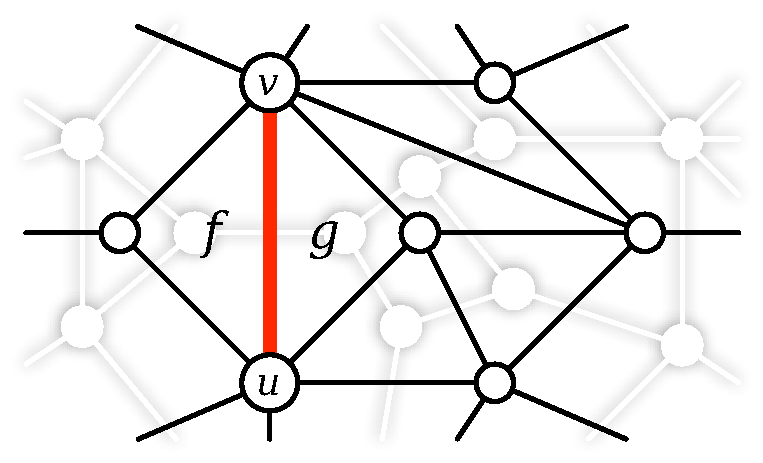
\includegraphics[height=0.9in]{Fig/primal}\quad
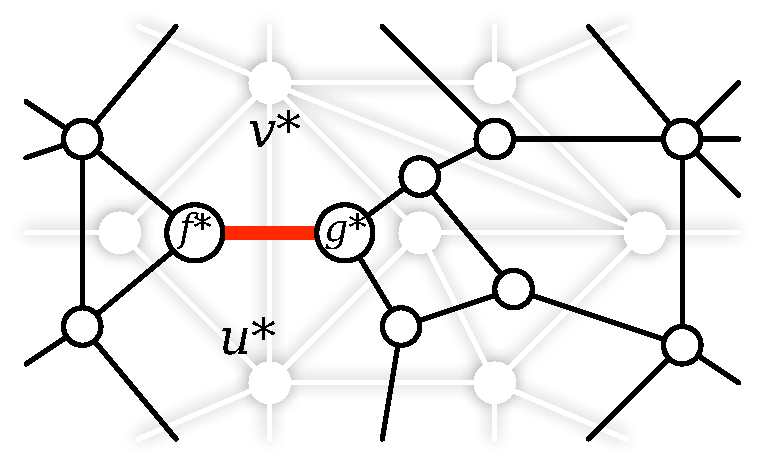
\includegraphics[height=0.9in]{Fig/dual}
\caption{Graph duality.  One edge $uv$ and its dual $(uv)^* =
f^*g^*$ are emphasized.} \label{fig:prelims_primaldual}
\end{figure}

Any undirected graph~$G$ embedded on a surface~$\Sigma$ without boundary has a
\EMPH{dual graph}~$G^*$, which has a vertex~$f^*$ for each face~$f$ of~$G$,
and an edge~$e^*$ for each edge~$e$ in~$G$ joining the vertices dual to the
faces of~$G$ that~$e$ separates. The dual graph~$G^*$ has a natural cellular
embedding in~$\Sigma$, whose faces corresponds to the vertices of~$G$.
See Figure~\ref{fig:prelims_primaldual}.
For any subgraph~${F = (U, D)}$ of~$G=(V,E)$, we write~$G \setminus F$
to denote the edge-complement~$(V,E \setminus D)$. We also abuse notation
by writing~$F^*$ to denote the subgraph of~$G^*$ corresponding to any
subgraph~$F$ of~$G$.
Further, we may sometimes use~$D$ to refer to an edge set or the subgraph~$F = (V, D)$,
but it should be clear which we mean from context.

A \EMPH{tree-cotree decomposition}~$(T,L,C)$ of an undirected
graph~$G$ embedded on a surface without boundary 
is a partition of the edges into three disjoint subsets;
a spanning tree~$T$ of~$G$, a spanning cotree~$C$ (the dual of a spanning
tree~$C^*$ of~$G^*$), and leftover edges~$L=G \setminus (T \cup C)$.
Euler's formula implies that in any tree-cotree decomposition, the set~$L$
contains exactly~$2g$ edges~\cite{e-dgteg-03}.
The definitions for dual
graphs and tree-cotree decompositions given above
extend to surfaces with boundary, but
we do not require these extensions in this dissertation.

For some of the problems we consider in Chapters~\ref{chap:non-trivial} and~\ref{chap:max-flow}, the input is actually a \emph{directed} edge-weighted (or capacitated)
graph~$G$ with a cellular embedding on some surface.
We use the
notation~$u \arcto v$ to denote the directed \EMPH{dart} from vertex~$u$ to vertex~$v$, and let~$\vec{E}$ be the set of darts in~$G$.
Without loss of generality, we consider only \EMPH{symmetric} directed graphs,
in which the reversal~$v \arcto u$ of any dart~$u \arcto v$ is another dart,
possibly with infinite weight (or~$0$ capacity).
We also assume that in the cellular embedding,
the images of any edge in~$G$ and its reversal coincide (but with opposite
orientations).
The two darts~$u \arcto v$ and~$v \arcto u$ therefore define an \EMPH{edge}~$uv$
with a canonical orientation~$u \arcto v$; edge~$vu$ does not necessarily exist even though~$uv$ does.
Thus, like Cabello \etal~\cite{ccl-fsncd-10} and Erickson~\cite{e-sncds-11},
we implicitly model directed graphs as \emph{undirected graphs with asymmetric
edge weights}.
We may denote dart~$u \arcto v$ as~$f \uparrow g$ if faces~$f$ and~$g$ lie to its left and right respectively.
The dual of any dart~$f \uparrow g$ is~$f^* \arcto g^*$.
Note that the duality of darts is \emph{not} an involution the way we have specified the orientation of the dual dart here.

Let~$p = v_0 \arcto v_1 \arcto \dots \arcto v_k$ be a simple directed cycle
or arc in an
embedded graph~$G$. We say an edge~$u \arcto v_i$ \EMPH{enters~$p$
from the left}
(resp. right) if the vertices~$v_{i-1}$,~$u$, and~$v_{i+1}$ (module~$k$
in the case of a cycle) are ordered
clockwise (resp. counterclockwise) around~$v_i$, according to the
embedding's rotation system. An edge~$v_i \arcto u$ \EMPH{leaves~$p$ from the
left} (resp. right) if its reversal~$u \arcto v_i$ enters~$p$ from the
left (resp. right).
If~$p$ is an arc,
the above definitions require that~$0 < i < k$ and that~$u$
is not a vertex in~$p$. Recall an arc's endpoints lie on boundary cycles.
Let~$t_0 v_0$ and~$v_0 w_0$ be the boundary edges
incident to~$v_0$ with vertices~$t_0$, $v_1$, and $w_0$ appearing in clockwise
order around~$v_0$. We say~$t_0 \arcto v_0$ enters~$p$ from the left.
We say~$w_0 \arcto v_0$ enters~$p$
from the right. Similarly,
if~$t_k v_k$ and~$v_k w_k$ are boundary edges incident to~$v_k$ with
vertices~$t_k$, $w_k$, and~$v_{k-1}$ appearing in clockwise order around~$v_k$,
we say~$t_k \arcto v_k$ enters~$p$ from the left and~$w_k \arcto v_k$
enters~$p$ from the right. Finally, we treat~$t_0$ as~$v_{-1}$ and~$t_k$
as~$v_{k+1}$ to define entering from the left (resp. right) for any
other edges~$u \arcto v_0$ or~$u \arcto v_k$ where~$u$ does not appear in~$p$.

\subsection{Homotopy and Homology}

Two paths~$p$ and~$q$ in $\Sigma$ are \EMPH{homotopic} if one can be
continuously deformed into the other without changing their endpoints.
More formally, a \EMPH{homotopy} between~$p$ and~$q$ is a
continuous map $h\colon {[0,1]\times [0,1] \to \Sigma}$ such that $h(0,\cdot) = p$, $h(1,\cdot) = q$, $h(\cdot, 0)=p(0)=q(0)$, and $h(\cdot,1)=p(1)=q(1)$.
Homotopy defines an equivalence relation over the set of paths with any
fixed pair of endpoints. The set of homotopy classes of loops in~$\Sigma$
with basepoint~$x_0$ defines a group~$\pi_i(\Sigma,x_0)$ under concatenation,
called the \EMPH{fundamental group} of~$\Sigma$. (For all basepoints~$x_0$
and~$x_1$, the groups~$\pi_i(\Sigma,x_0)$ and~$\pi_i(\Sigma,x_1)$ are
isomorphic.) A cycle is \EMPH{contractible} if it is homotopic to a constant
map.
Given a weight function on the darts of~$G$, we say a directed path or cycle is \EMPH{tight} if it has minimum total weight (counting edges with multiplicity) for its homotopy class.

Homology is a coarser equivalence relation than homotopy, with nicer
algebraic properties.  Like several earlier papers \cite{cf-qhc2-07,
cf-qhc-08, dls-chtl-07, dlsc-cgaht-08}, we will consider only
one-dimensional cellular homology with coefficients in the finite
field $\Z_2$; this restriction allows us to radically simplify our
definitions.  For a more general treatment of homology, we refer the
reader to our companion paper~\cite{cen-hfcc-09} or to standard
references on topology \cite{h-at-01, s-ctcgt-93, z-tc-05}.

%\note{Reviewer 2 suggests: "you should probably emphasize that the even and boundary subgraphs are vector spaces over $Z_2$, and define $\oplus$."}

Fix a cellular embedding of an undirected graph $G$ on a surface with genus $g$ and $b$ boundaries.  An \EMPH{even subgraph} is a subgraph of $G$ in which every node has even degree, or equivalently, the union of edge-disjoint cycles.  A \EMPH{boundary subgraph} is the boundary of the union of a subset of faces of $G$; for example, every separating cycle is a boundary subgraph.
%For planar graphs, every even subgraph is a boundary subgraph, but this equivalence does not extend to higher-genus embeddings.
Two even subgraphs are \EMPH{homologous}, or in the same \EMPH{homology class}, if their symmetric difference is a boundary subgraph.
%Equivalently, two even subgraphs are homologous if one can be continuously deformed into the other via a deformation that may include splitting cycles at self-intersection points, merging intersecting pairs of cycles, or adding or deleting contractible cycles.
Boundary subgraphs are also called \EMPH{null-homologous}.  Any two homotopic cycles are homologous, but homologous cycles are not necessarily homotopic; see Figure \ref{F:homology}.  Moreover, the homology class of a cycle can contain even subgraphs that are not cycles; see Figure \ref{F:homology2}.

%\note{Reviewer 2 says: "Figure 1, left, is hard to understand (draw the hidden parts of the curves".  Erin: I disagree!  I wouldn't change it, but that's your call, Jeff.}

%\note{Jeff: Um.  The `hidden' parts of the curves are already there: thinner, lighter, and cased.  I don't know how to make them any clearer!  The lack of visualization ability in the SOCG community never ceases to amaze me.}

\begin{figure}[htb]
\centering
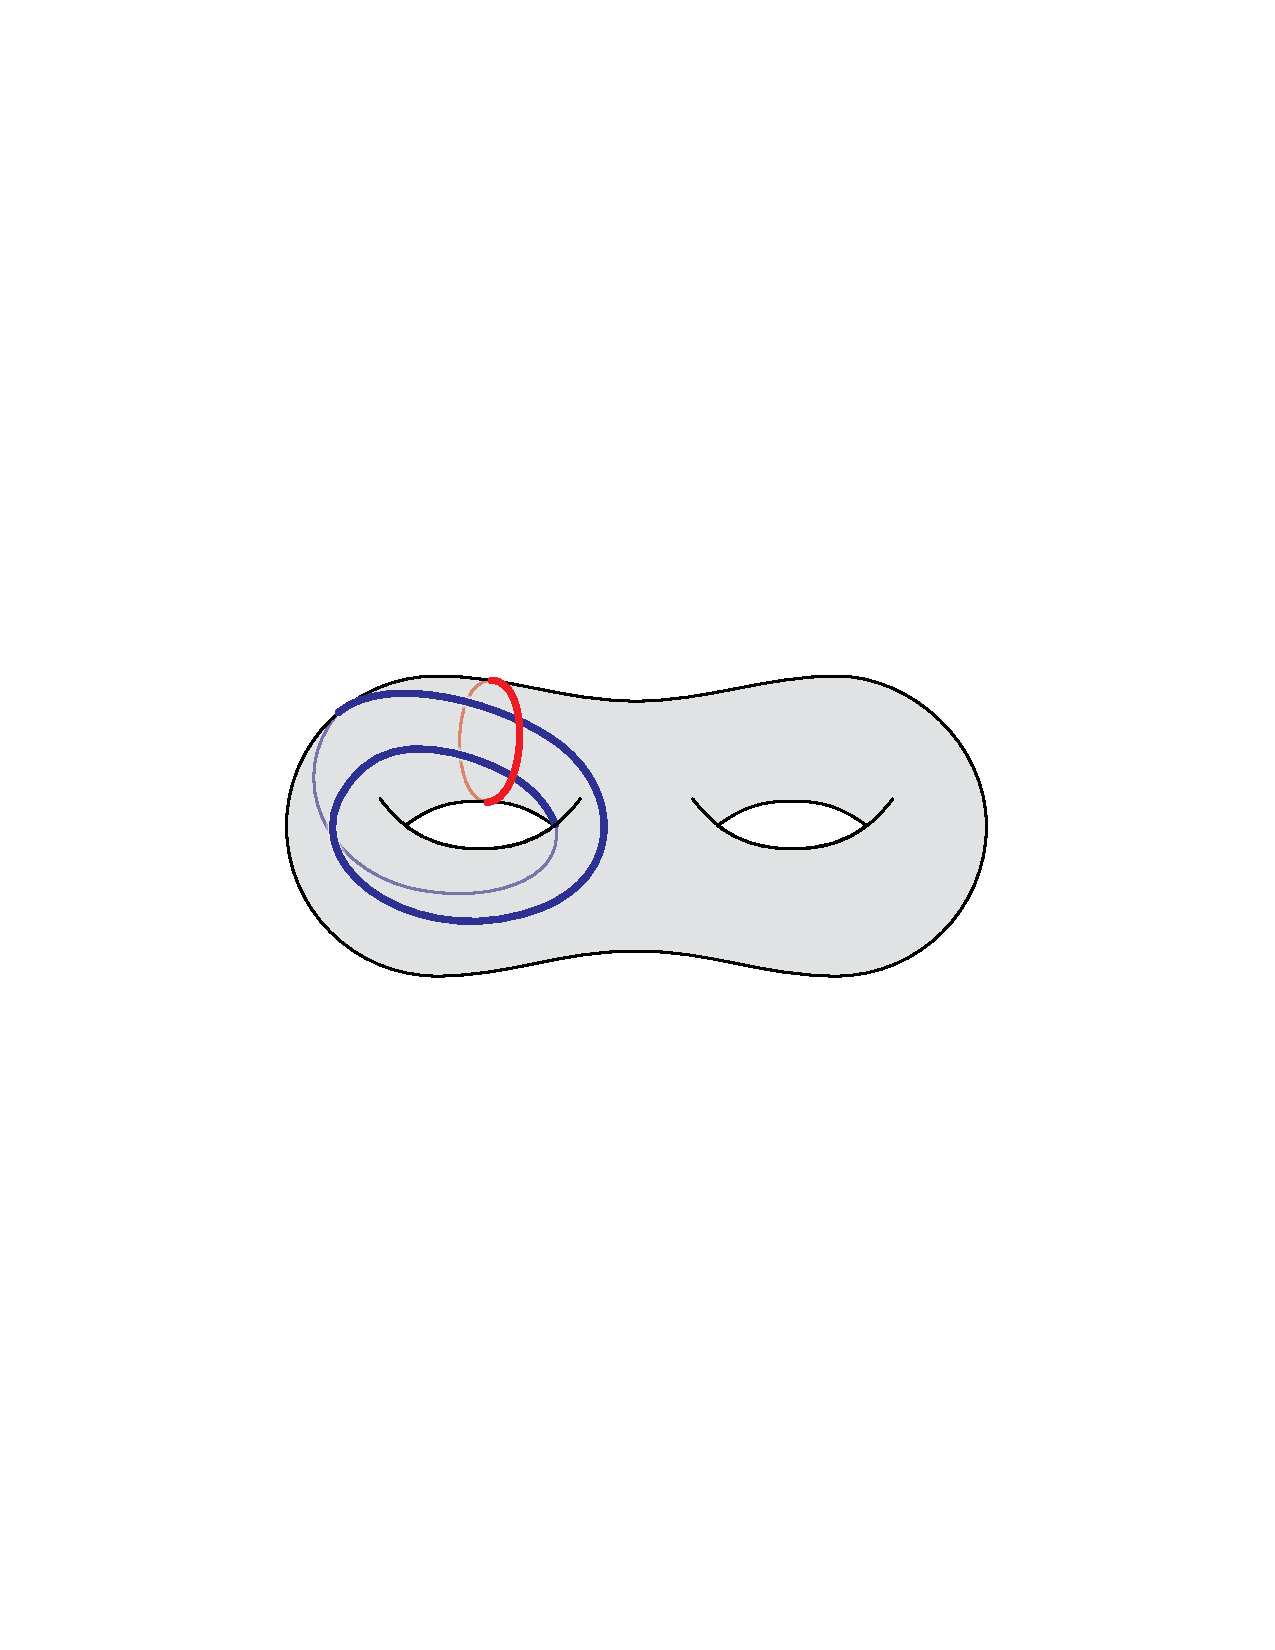
\includegraphics[height=0.75in]{Fig/homologous3}\\[2ex]
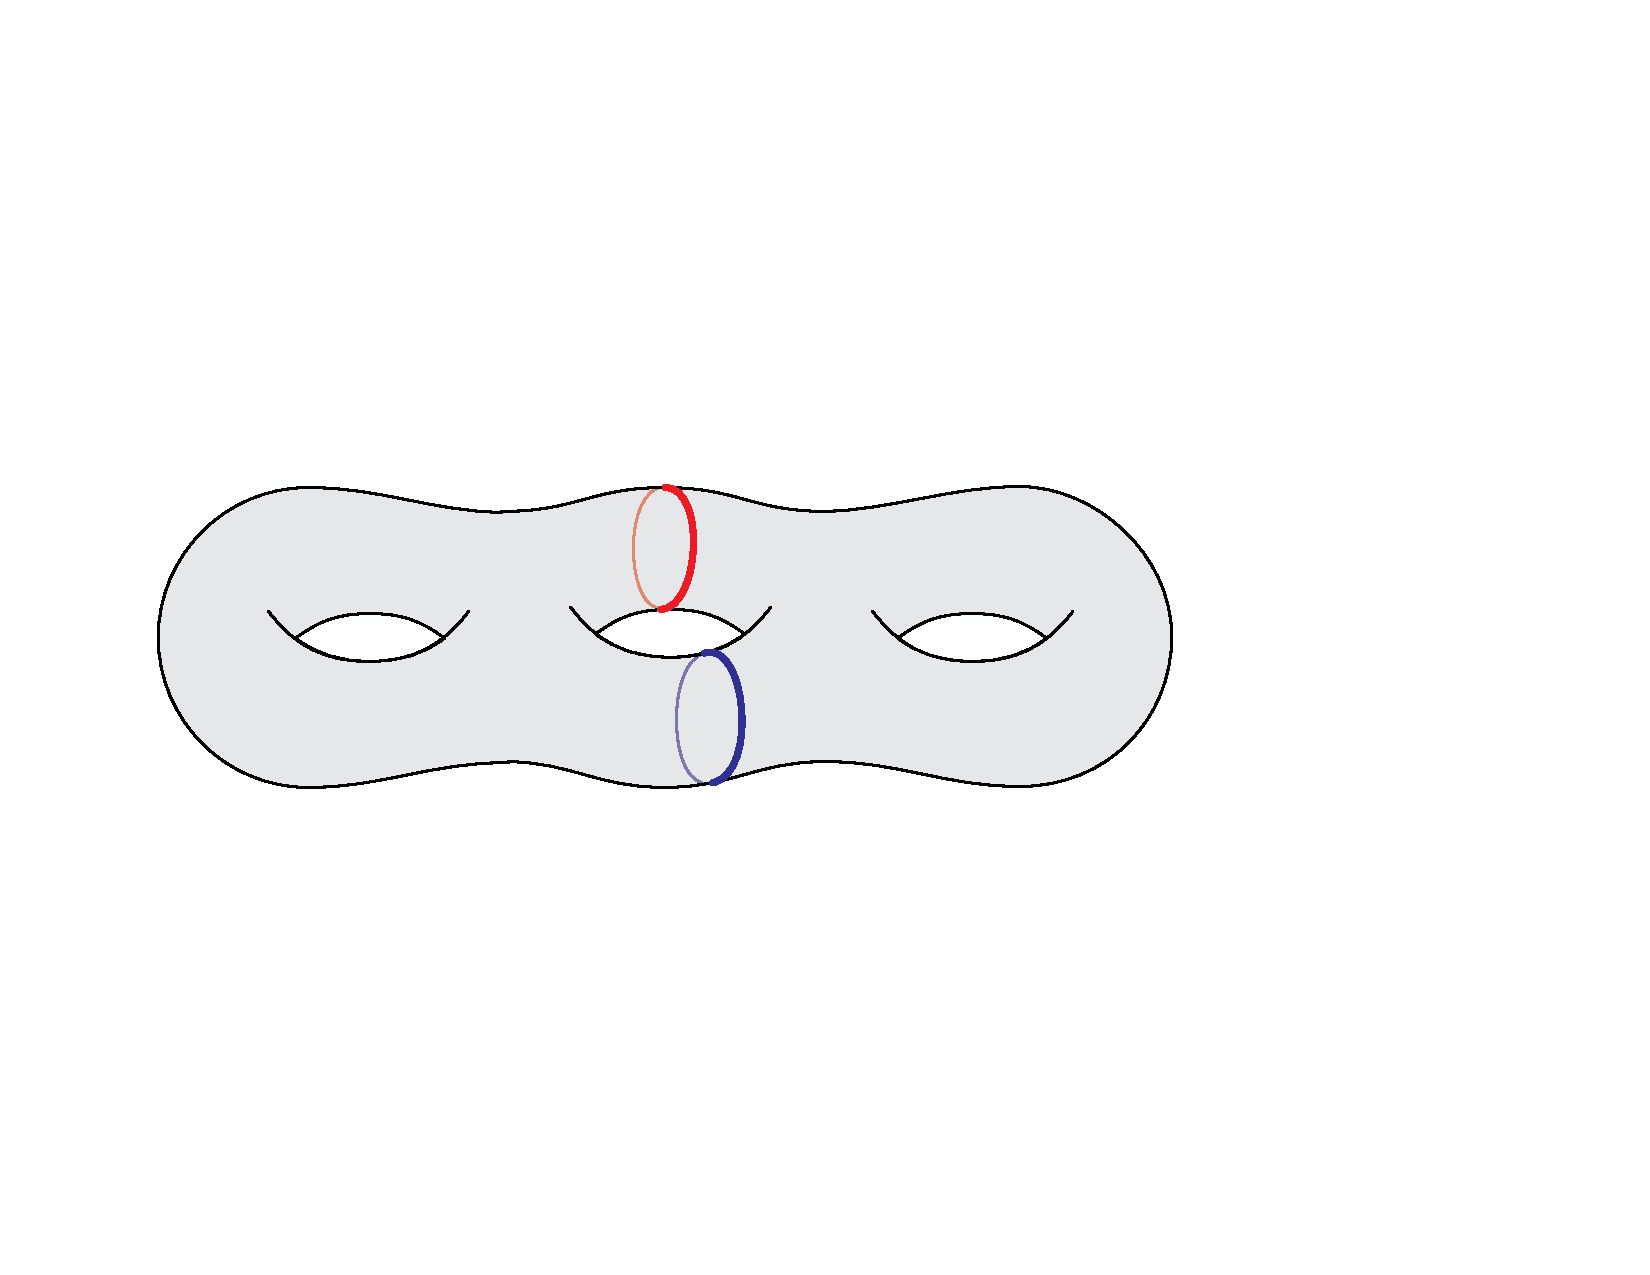
\includegraphics[height=0.75in]{Fig/homologous2}
\caption{Homologous pairs of cycles that are not homotopic.  (Lighter portions of the curves are on the back side of the surface.)}
\label{F:homology}
\end{figure}

\begin{figure}[htb]
\centering
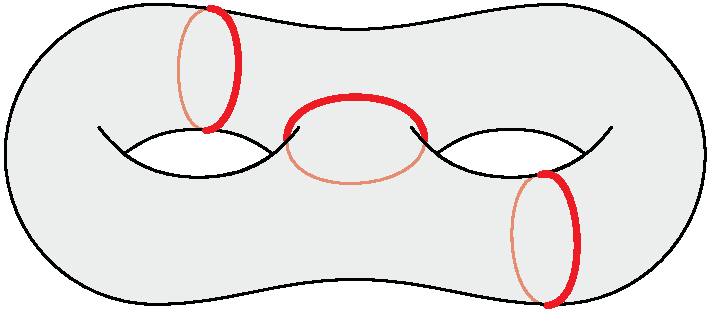
\includegraphics[height=0.75in]{Fig/homologous1}
\caption{Each cycle is homologous to the union of the other two.}
\label{F:homology2}
\end{figure}

\subsection{Flows and Cuts}
Consider again homology with coefficients in~$\R$.
We will often refer to $1$-chains as \EMPH{flows} or \EMPH{coflows} depending on if we are focusing on the primal or dual graph.
Any flow can be decomposed to a set of weighted paths and cycles.
For any capacity function~$c : \vec{E} \to \R$ on the \emph{darts}, we say a flow~$\phi$ is \EMPH{feasible} if $-c(v \arcto u) \leq \phi(uv) \leq c(u \arcto v)$.
Note that capacity functions do not necessarily have to be non-negative for feasibility to be well defined.
Given a coflow~$\theta$ we define the capacity of~$\theta$ with respect to~$c$ as follows.
Let~$c' : E \to \R$ be a function on the edges such that~$c'(uv) = c(u \arcto v)$ if~$\theta(uv) \geq 0$ and~$c'(uv) = -c(v \arcto u)$ if~$\theta(uv) < 0$.
The capacity of~$\theta$ with respect to~$c$ is the dot product~$\langle \theta, c' \rangle$.

For $s,t \in V$, an $s,t$-\EMPH{flow} is a 1-chain $\phi: E \to \R$ such that $\partial \phi(v) = 0$ for all $v \in V\backslash \{s,t\}$.
The value of an $s,t$-flow~$\phi$ is $\sum_{s \arcto v} \phi(s \arcto v)$.
A \EMPH{maximum $s,t$-flow} with respect to a capacity function~$c$ is a feasible flow of highest value.
For a flow $\phi$, the \EMPH{residual capacity} function $c_{\phi}: \vec{E} \to \R$ is defined as $c_{\phi}(u \arcto v) = c(u \arcto v) - \phi(u \arcto v)$.
Given a capacity function~$c$, we may refer to the \EMPH{residual graph $G_{\phi}$} when discussing the graph~$G$ coupled with residual capacity function~$c_\phi$.
The \EMPH{dual residual graph}~$G^*_{\phi}$ is simply the dual graph~$G^*$ coupled with the residual capacity function~$c_\phi$.

An \EMPH{cut} in~$G = (V, E)$ is defined as a subset of vertices~$S \subseteq V$; we refer to $S$ and $T = V\backslash S$ as different \EMPH{sides} of the cut.
Given two vertices~$s$ and~$t$ with $s \in S$ and $t \in T$, we say $S$ is an
\EMPH{$s,t$-cut}.
A dart~$u \arcto v$ (and its associated edge~$uv$ or~$vu$) \EMPH{crosses} a cut $S$ if exactly one of $u$ and $v$ lie in $S$.
In particular, $u \arcto v$ crosses $S$ in the \EMPH{forward} direction if $u\in S$ and in the \EMPH{backward} direction if $v \in S$.
For a cut $S$ we use the notation \EMPH{$\Gamma^+(S)$} to denote the set of all darts that cross $S$ in the \emph{forward} direction.
We define \EMPH{$\Gamma^-(S)$} as the set of darts that cross $S$ in the backward direction.
A walk $W$ crosses a cut $S$ $k$ times if  there are $k$ edges of $W$ that cross $S$.

Given a dart capacity function~$c : \vec{E} \to \R$, the value or capacity of a cut~$S$ is~$\sum_{u \arcto v \in \Gamma^+(S)} c(u \arcto v)$.
Equivalently, the capacity of a cut~$S$ is equal to the capacity of a coflow~$\theta$ such that~$\theta(u \arcto v) = 1$ if~$u \arcto v \in \Gamma^+(S)$ and~$\theta(u \arcto v) = 0$ if~$uv$ does not cross~$S$.
A \EMPH{minimum $s,t$-cut} of~$G$ with respect to capacity function~$c$ is an $s,t$-cut of minimum value.
The well known maximum-flow/minimum-cut theorem of Ford and Fulkerson~\cite{ff-mfn-56} states that for any non-negative capacity function $c$, the value of a maximum feasible $s,t$-flow is equal to the value of a minimum $s,t$-cut.


\subsection{Covering Spaces and Cutting}

A continuous map~$\pi : \Sigma' \to \Sigma$ between two surfaces is called a
\EMPH{covering map} if each point~$x \in \Sigma$ lies in an open
neighborhood~$U$ such that (1)~$\pi^{-1}(U)$ is a countable union of disjoint
open sets~$U_1 \cup U_2 \cup \cdots$ and (2) for each~$i$, the
restriction~$\pi |_{U_i} : U_i \to U$ is a homeomorphism. If there is a covering
map~$\pi$ from~$\Sigma'$ to~$\Sigma$, we call~$\Sigma'$ a \EMPH{covering space}
of~$\Sigma$. The \EMPH{universal cover}~$\tilde{\Sigma}$ is the unique
simply-connected covering space of~$\Sigma$ (up to homeomorphism).
The universal cover is so named because it covers every path-connected
covering space of~$\Sigma$.

For any path~$p : [0,1] \to \Sigma$ such that~$\pi(x') = p(0)$ for some
point~$x' \in \Sigma'$, there is a unique path~$p'$ in~$\Sigma'$, called
a \EMPH{lift} of~$p$, such that~$p'(0) = x'$ and~$\pi \circ p' = p$. We also
say that~$p$ \EMPH{lifts} to~$p'$. Conversely, for any path~$p'$ in~$\Sigma'$,
the path~$\pi \circ p'$ is called a \EMPH{projection} of~$p'$.

We define a lift of a cycle~$\gamma : S^1 \to \Sigma$ to be the infinite
path~$\gamma' : \R \to \Sigma'$ such that
${\pi(\gamma'(t)) = \gamma(t \mod 1)}$
for all real~$t$. We call the path obtained by restricting~$\gamma'$ to any
unit interval a \EMPH{single-period lift} of~$\gamma$; equivalently, a
single-period lift of~$\gamma$ is a lift of any loop equivalent to~$\gamma$.
We informally say that a cycle is the~\EMPH{projection} of any of its
single-period lifts.

\EMPH{Cutting} a combinatorial surface along a cycle or  arc modifies both the surface and the embedded graph.
For any combinatorial surface $S = (\Sigma, G)$ and any simple cycle or arc $\gamma$ in~$G$, we define a new combinatorial surface \EMPH{$S \snip \gamma$} by taking the topological closure of $\Sigma \backslash \gamma$ as the new underlying surface; the new embedded graph contains two copies of each vertex and edge of $\gamma$, each bordering a new boundary.
Similar to covering spaces, we define the~\EMPH{projection} of a curve in~$S \snip \gamma$ as the natural mapping of points (or vertices and edges) to~$S$.

\section{Characterizing Homology}
\label{sec:characterizing}

Throughout the paper, we fix a directed graph $G=(V,E)$, a non-negative weight function $w\colon E\to \Real$, and a cellular embedding of $G$ on a surface $\Sigma$ of genus $g$ with $b$ boundaries.
When considering undirected graphs, we assume the weight function is symmetric.
Without loss of generality, we assume that the underlying surface $\Sigma$ has at least one boundary; otherwise, we can remove an arbitrary face of $G$ from~$\Sigma$ without affecting its homology at all.  Let $\delta_1, \dots, \delta_b$ denote the boundary cycles of $\Sigma$, and let $\beta = 2g+b-1$ denote the the first Betti number of $\Sigma$.

In this section, we describe two standard methods for preprocessing a combinatorial surface in~$O(\beta n)$ time, so that the $\Z_2$-homology class of any even subgraph $\eta$ can be computed in $O(\beta)$ time per edge.
Both methods characterize the homology class of any even subgraph using a vector of~$\beta$ bits.
The vectors are computed using a one of two natural generalizations of tree-cotree decompositions~\cite{e-dgteg-03} to surfaces with boundary.
In the first method, the vector is based on the crossings between~$\eta$ and a set of~$\beta$ primal paths.
By carefully selecting these paths, we can place a bound on the number of times a~$\Z_2$-minimal even subgraph can cross any of these paths; this bound is necessary for the algorithm given in Section~\ref{sec:crossing}.
In the second method, the vector is based on the crossings between~$\eta$ and a set of~$\beta$ \emph{dual} paths.
The vectors from the second method are more easily described and computed than the ones in the first, so we opt to use the second method in the algorithm given in Section~\ref{sec:homcover}.



\subsection{Crossing parity vectors}

The first method begins by computing a set $P$ of~$\beta$ paths, each of which is the concatenation of two shortest paths (possibly meeting in the interior of an edge), such that the surface $\Sigma\setminus P$ is a topological disk.
Specifically, it constructs a \emph{greedy system of arcs} in $O(\beta n)$ time, using a modification by Chambers \etal~\cite{ccelw-scsih-08} to an algorithm of Erickson and Whittlesey~\cite{ew-gohhg-05} for constructing a \emph{greedy system of loops}.
If the surface has exactly one boundary, then the greedy system of arcs is identical to a greedy system of loops where every loop shares the same basepoint on the boundary.
\note{TODO(kylejfox): Explicitly describe the construction using Henzinger \etal for the shortest paths.}

Let $p_1, p_2, \dots, p_\beta$ denote the paths in $P$.  It is no coincidence that the number of paths in $P$ is equal to the dimension of the homology group $H(G)$.  Indeed, we can identify the homology class of any even subgraph by considering the number of times it crosses each path in $P$, as follows.

For any cycle $\gamma$ and any index $i$, let $x_i(\gamma)$ denote the number of times $\gamma$ crosses the path~$p_i$.  The \EMPH{crossing vector} $x(\gamma)$ is the vector $(x_1(\gamma), \dots, x_\beta(\gamma))$.  The crossing vector of a set of cycles is the sum of the crossing vectors of its elements.
\begin{lemma}
\label{lem:decomposition}
Every even subgraph of an embedded graph has a cycle decomposition.
\end{lemma}

\begin{proof}
Let $H$ be an even subgraph of $G$.  We can decompose $H$ into cycles by specifying, at each vertex $v$, which pairs of incident edges of $H$ are consecutive.  Any pairing that does not create a crossing at $v$ is sufficient.  For example, if $e_1, e_2, \dots, e_{2d}$ are the edges of $H$ incident to $v$, indexed in clockwise order around $v$, we could pair edges $e_{2i-1}$ and $e_{2i}$ for each $i$.  
\end{proof}

Crossing vectors are not well-defined for arbitrary even subgraphs; different cycle decompositions can yield different crossing numbers.  However, the \emph{parity} of the crossing numbers is independent of the cycle decomposition.  The \EMPH{crossing parity vector} of any even subgraph $H$ is the bit vector $\bar{x}(H) = (\bar{x}_1, \dots, \bar{x}_\beta)$, where $\bar{x}_i = 1$ if the path $p_i$ crosses (any cycle decomposition of) $H$ an odd number of times, and $\bar{x}_i = 0$ otherwise.

\begin{lemma}
Two even subgraphs are $\Z_2$-homologous if and only if their crossing parity vectors are equal.
\end{lemma}

\begin{proof}
Every boundary subgraph is the symmetric difference of facial cycles.  Any non-contractible loop or arc crosses any facial cycle an even number of times; thus, the crossing parity vector of any facial cycle is the zero vector.  Every pair of even subgraphs $H$ and $H'$ satisfies the identity $x(H\oplus H') = x(H) \oplus x(H')$.  Thus, the crossing parity vector of any boundary subgraph is the zero vector.
\end{proof}

\begin{lemma}
We can compute the crossing parity vector of any even subgraph in $O(\beta)$ time per edge after computing~$P$.
\end{lemma}

\begin{proof}
We can compute a cycle decomposition $\gamma_1, \dots, \gamma_r$ of $H$ in $O(1)$ time per edge, by following the proof of Lemma~\ref{lem:decomposition}.
We can compute the number of crossings between any cycle $\gamma_i$ and any path $p_j$ in time proportional to the number of edges in $\gamma_i$.
\end{proof}



\subsection{Homology signatures}

Our second method associates a vector of $\beta$ bits with each edge $e$, called the \EMPH{signature} of~$e$; the homology class of any even subgraph is characterized by the bit-wise exclusive-or of the signatures of its edges.

Again, our construction is based on one of two natural generalizations of tree-cotree decompositions~\cite{e-dgteg-03} to surfaces with boundary; the second generalization is used for computing crossing parity vectors in the first method described above and is used in Section \ref{sec:homcover}.
We define a \EMPH{tree-coforest decomposition} of $G$ to be any partition $(T, F, X)$ of the edges of $G$ into three edge-disjoint subgraphs with the following properties:
\begin{itemize}\itemsep0pt
\item $T$ is a spanning tree of $G$.
\item $F^*$ is a spanning \emph{forest} of $G^*$, that is, an acyclic subgraph that contains every vertex.
\item Each component of $F^*$ contains a single dual boundary vertex $\delta_i^*$.
\end{itemize}
Euler's formula implies that there are exactly $\beta$ edges in $X$; arbitrarily index these edges $e_1, \dots, e_\beta$.  For each edge $e_i\in X$, adding the corresponding dual edge $e_i^*$ to $F^*$ creates a new dual path $\dualarc_i$, which is either a simple path between distinct boundary vertices, or a nontrivial loop from a boundary vertex back to itself; in the second case, $\dualarc_i$ may traverse some edges of $F^*$ twice.  We can treat each path $\dualarc_i$ as a simple arc in the \emph{abstract} surface $\Sigma$; cutting along these $\beta$ arcs transforms $\Sigma$ into a topological disk.
See Figure \ref{fig:tree-coforest}.

\begin{figure}[htb]
\centering\footnotesize\sf
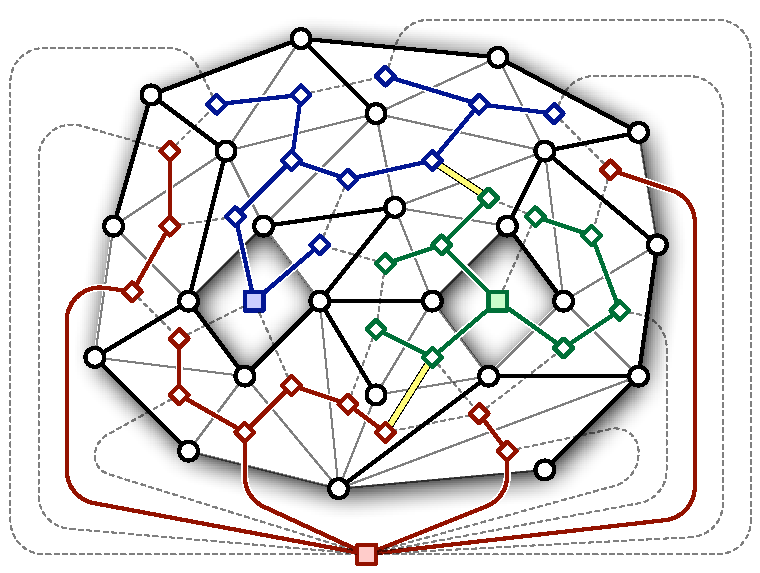
\includegraphics[scale=0.45]{Fig/tree-coforest2} \qquad
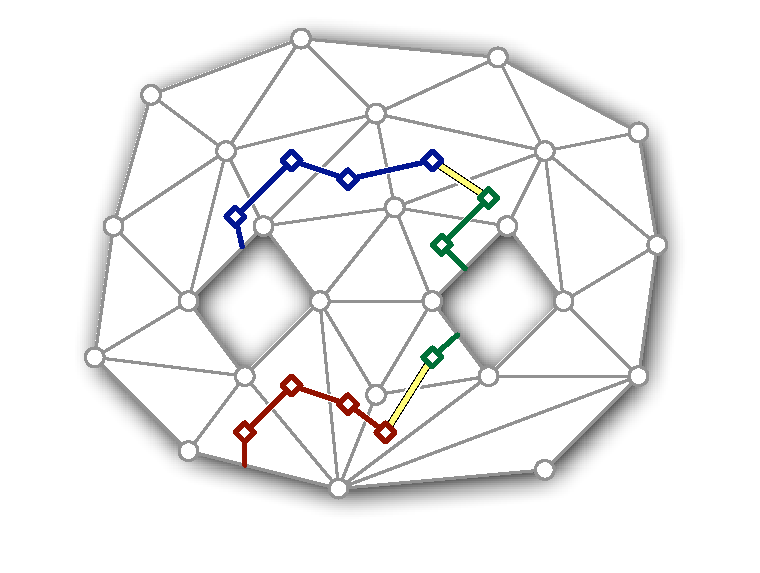
\includegraphics[scale=0.45]{Fig/tree-coforest-arcs2}
\caption{Left: A tree-coforest decomposition of the graph in Figure~\ref{fig:duality}; doubled lines indicate edges in $X$.
Right: The resulting system of dual arcs.  Compare with Figure \ref{fig:forest-cotree}.}
\label{fig:tree-coforest}
\end{figure}

Finally, for each edge $e$ in $G$, we define its signature \EMPH{$[e]$} to be the $\beta$-bit vector whose $i$th bit is equal to $1$ if and only if $e$ crosses $\dualarc_i$ (that is, if $\dualarc_i$ traverses the dual edge $e^*$) exactly once.  The signature $[\eta]$ of an even subgraph $\eta$ is the bitwise exclusive-or of the signatures of its edges.  Similarly, the signature~$[\cycle]$ of a cycle $\cycle$ is the bitwise exclusive-or of the signatures of the edges that $\cycle$ traverses an odd number of times.

Let \EMPH{$h \oplus h'$} denote the bitwise exclusive-or of two homology signatures $h$ and $h'$, or equivalently, their sum as elements of the homology group~$(\Z_2)^\beta$.  The identities $[\eta \oplus \eta'] = [\eta] \oplus [\eta']$ and $[\cycle\cdot\cycle'] = [\cycle] \oplus [\cycle']$ follow directly from the definitions.

\begin{lemma}
\label{lem:sign}
We can preprocess $G$ in $O(\beta n)$ time, so that the signature $[\cycle]$ of any cycle can be computed in $O(\beta)$ time per edge.
\end{lemma}

\begin{proof}
A tree-coforest decomposition can be computed in $O(n)$ time as follows.  First construct a graph~$H$ by identifying all the dual boundary vertices in $G^*$ to a single vertex.  Compute a spanning tree of $H$ by whatever-first search; the edges of this spanning tree define an appropriate dual spanning forest~$F^*$.  Construct the subgraph $G\setminus F$ and compute a spanning tree $T$ via whatever-first search.  Finally, let $X = G\setminus (T\cup F)$.  With the decomposition in hand, it is straightforward to compute each path $\dualarc_i$ in $O(n)$ time, and then compute each edge signature in $O(\beta)$ time.
\end{proof}

\begin{lemma}
An even subgraph $\eta$ of $G$ is null-homologous in $\Sigma$ if and only if $[\eta] = 0$.
\end{lemma}

\begin{proof}
Let $\eta$ be a null-homologous even subgraph of $G$.  Then by definition, $\eta$ is the boundary of the union of a subset~$Y$ of faces of $G$.  The boundary of any face $f$ is contractible in $\Sigma$ and therefore has signature $0$.  It follows immediately that $[\eta] = [\bigoplus_{f\in Y} \partial f] = \bigoplus_{f\in Y} [\partial f] = 0$.

Conversely, suppose $\eta$ crosses each arc $\dualarc_i$ an even number of times, so $[\eta]=0$.  Let $x$ and $y$ be two intersection points between $\eta$ and some arc $\dualarc_i$, and let $\dualarc_i[x,y]$ be the subpath of $\dualarc_i$ between those two points.  Replacing tiny segments of $\eta$ through~$x$ and~$y$ with two copies of $\dualarc_i[x,y]$ does not change the homology class of $\eta$, but does reduce the number of intersection points between $\eta$ and $\dualarc_i$.  It follows by induction that~$\eta$ is homologous to another even graph $\eta'$ that does not intersect any path~$\dualarc_i$ at all.  This even graph lies entirely within the disk $\Sigma\setminus \bigcup_i\dualarc_i$, and is therefore null-homologous.
\end{proof}


The following corollaries are now immediate.

\begin{corollary}
Two even subgraphs $\eta$ and $\eta'$ of $G$ are $\Z_2$-homologous in $\Sigma$ if and only if $[\eta] = [\eta']$.
\end{corollary}

\begin{corollary}
Two cycles $\cycle$ and $\cycle'$ in $G$ are $\Z_2$-homologous in $\Sigma$ if and only if $[\cycle] = [\cycle']$.
\end{corollary}

\section{Crossing Sequences and Triangulations}

\note{TODO: Write a section on computing $\Z_2$-minimal even subgraphs (and cycles?) using the SoCG 2009 crossing sequence method.}

\section{The $\Z_2$-Homology Cover}
\label{sec:homcover}

Now, let~$G$ be directed, and let $h$
be a homology signature.  In this section, we describe an
algorithm to compute a $\Z_2$-minimal \emph{cycle} with signature~$h$
in $(g+b)^{O(g+b)}n \log n$ time. Our algorithm can be
used as a subroutine to compute minimum-cost even subgraphs in
\emph{any} homology class in the same asymptotic running time
using a dynamic programming procedure described later in this section.
Again, by Lemma~\ref{lem:surface-st-cut}, our algorithm can be used to find a minimum $s,t$-cut in~$G^*$ in the same amount of time if~$G$ is undirected.

The algorithm of the previous section constructs and searches several relevant finite portions of the (infinite) universal cover of the input surface.
Instead of the universal cover, the algorithms of this section construct and search another canonical covering space, called the \emph{$\Z_2$-homology cover}.
We also use a generalization of Klein's seminal multiple-source shortest path algorithm~\cite{k-msspp-05} for planar graphs to higher-genus embedded graphs \cite{cce-msspe-13}.
\note{TODO(kylejfox): The top of page 2 in the SODA 2011 paper contains some good motivation for the homology cover technique. That material should be transferred either to here or the introduction. Also mention the shortest non-trivial directed cycle papers~\cite{e-sncds-11,f-sntcd-13} that use similar techniques.}

\subsection{Constructing the $\Z_2$-homology cover}
\label{sec:homcover_cover}
After computing homology signatures for each edge, the $\Z_2$-homology cover of a combinatorial surface can be defined using a standard~\emph{voltage construction}~\cite[Chapter 4]{gt-tgt-01}, as follows.  Let $\Gbar$ denote the graph whose vertices are all ordered pairs $(v, h)$ where $v$ is a vertex of $G$ and $h$ is an element of $(\Z_2)^\beta$, and whose edges are the ordered pairs $(\arc{u}{v}, h) := (u, h)\arcto(v, h\oplus [u\arcto v])$ for all edges $\arc{u}{v}$ of $G$ and all homology classes $h \in (\Z_2)^\beta$.  Let $\pi\colon \Gbar\to G$ denote the covering map $\pi(v, h) = v$; this map projects any cycle in $\Gbar$ to a cycle in $G$.  To define a cellular embedding of~$\Gbar$, we declare a cycle in $\Gbar$ to be a face if and only if its projection is a face of $G$.  The combinatorial surface defined by this embedding is the $\Z_2$-homology cover $\Sigmabar$.

Our construction can be interpreted more topologically as follows.  Let $\dualarc_1, \dots, \dualarc_\beta$ denote the system of dual arcs used to define the homology signatures $[e]$.  The surface $D := \Sigma\setminus(\dualarc_1\cup\cdots\cup \dualarc_\beta)$ is a topological disk.  Each arc $\dualarc_i$ appears on the boundary of $D$ as two segments $\dualarc^+_i$ and~$\dualarc^-_i$.  For each signature $h\in (\Z_2)^\beta$, we create a disjoint copy $(D,h)$ of $D$; for each index~$i$, let $(\dualarc^+_i, h)$ and $(\dualarc^-_i, h)$ denote the copies of $\dualarc^+_i$ and $\dualarc^-_i$ in the disk $(D, h)$.  For each index~$i$, let~$b_i$ denote the $\beta$-bit vector whose $i$th bit is equal $1$ and whose other $\beta-1$ bits are all equal to~$0$.  The $\Z_2$-homology cover $\Sigmabar$ is constructed by gluing the~$2^\beta$ copies of $D$ together by identifying boundary paths $(\dualarc^+_i,h)$ and $(\dualarc^-_i, h\oplus b_i)$, for every index $i$ and homology class $h$.  See Figure \ref{fig:cover-ex} for an example.

\begin{figure}
\centering
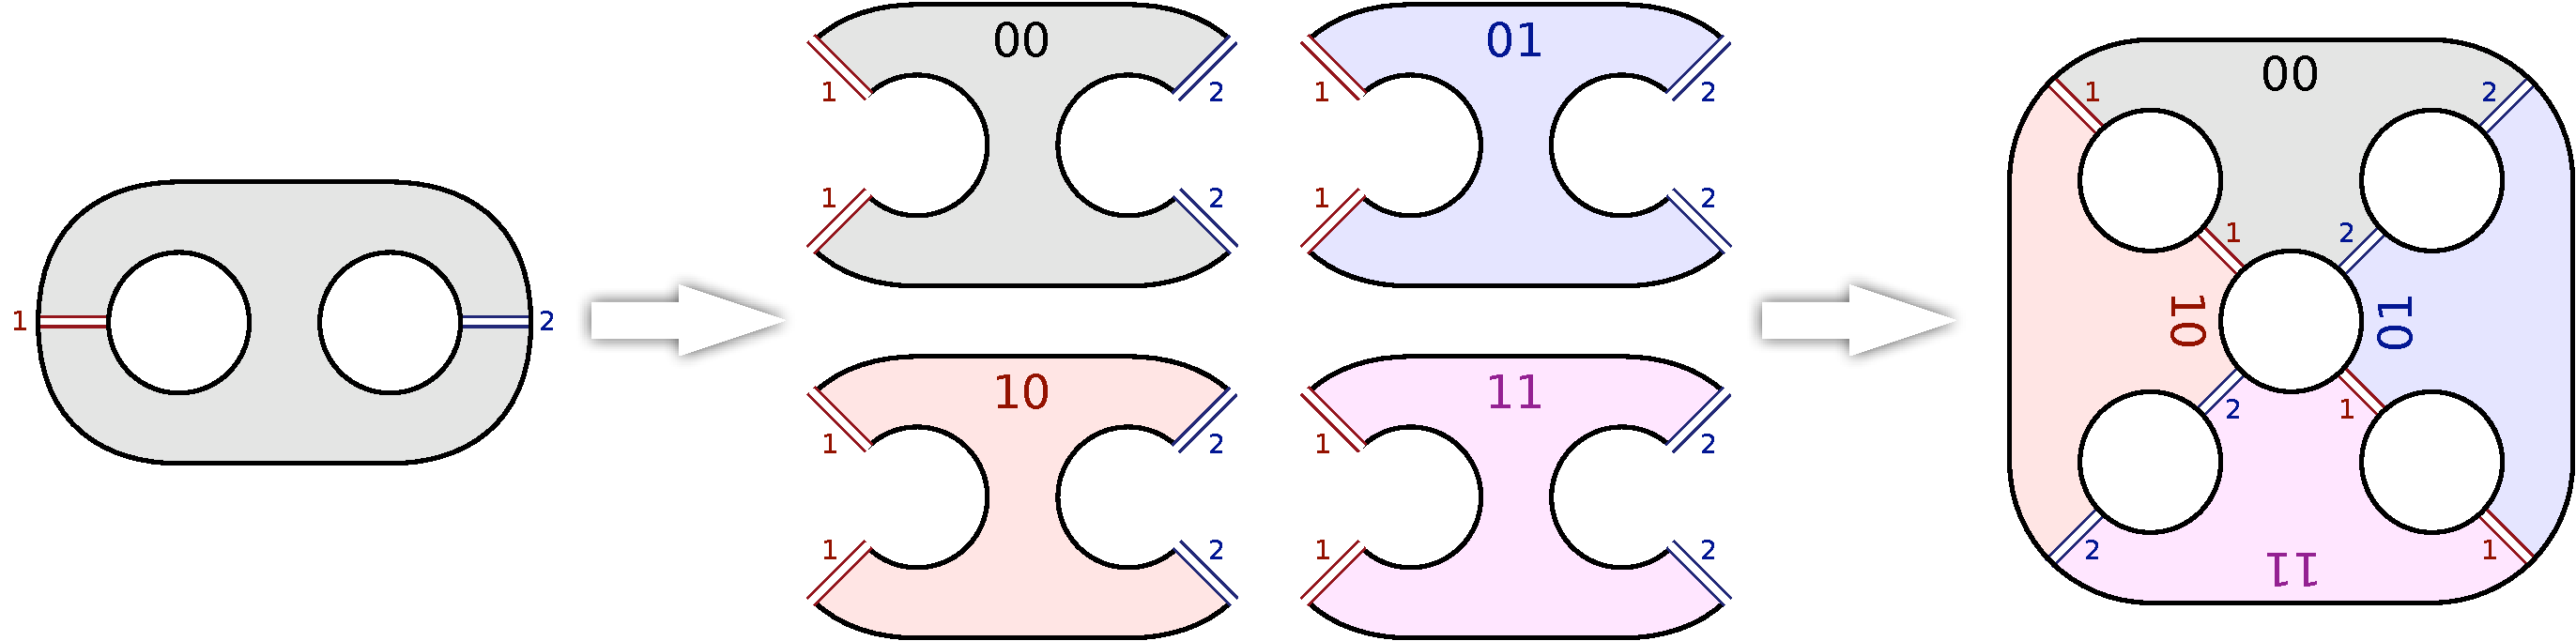
\includegraphics[height=1.5in]{Fig/hom-cover-example}
\caption{Constructing the $\Z_2$-homology cover of a pair of pants (a genus zero surface with three boundaries).}
\label{fig:cover-ex}
\end{figure}

\begin{lemma}
\label{lem:cover-cxy}
The combinatorial surface $\Sigmabar$ has $\nbar = 2^\beta n$ vertices, genus $\gbar = O(2^\beta \beta)$, and $\bbar = O(2^\beta b)$ boundaries, and it can be constructed in $O(2^\beta n)$ time.
\end{lemma}

\begin{proof}
Let $m$ and $f$ denote the number of edges and faces of $\Sigma$, respectively.  Recall that the Euler characteristic of $\Sigma$ is $\chi = n - m + f = 2 - 2g - b = 1-\beta$.  The combinatorial surface~$\Sigmabar$ has exactly $\nbar = 2^\beta n$ vertices, $2^\beta m$ edges, and $2^\beta f$ faces, so its Euler characteristic is $\chibar = 2^\beta (1-\beta)$.

If $b>1$, then each boundary cycle $\delta_i$ has a non-zero homology signature; at least one arc $\dualarc_j$ has exactly one endpoint on~$\delta_i$.  Thus, $\Sigmabar$ has exactly $\bbar = 2^{\beta-1} b$ boundary cycles, each of which is a double-cover (in fact, the $\Z_2$-homology cover) of some boundary cycle~$\delta_i$.  It follows that~$\Sigmabar$ has genus $\gbar = 1-(\chibar+\bbar)/2 = {2^{\beta-2} ({4g+b-4}) + 1}$.  (Somewhat surprisingly, $\Sigmabar$ may have positive genus even when $\Sigma$ does not!)  On the other hand, when $b=1$, the boundary cycle~$\delta_1$ is null-homologous, so $\Sigmabar$ has $\bbar = 2^\beta b$ boundary cycles, and thus~$\Sigmabar$ has genus $\gbar = {1-(\chibar+\bbar)/2} =  {2^\beta (g-1) + 1}$.

After computing the homology signatures for $\Sigma$ in $O(\beta n)$ time, following Lemma \ref{lem:sign}, it is straightforward to construct $\Sigmabar$ in $O(\nbar) = O(2^\beta n)$ time.
\end{proof}

We assign weights to the directed edges of $\Gbar$ by setting $\wbar(\arc{u}{v},h) := w(\arc{u}{v})$ for each edge $\arc{u}{v}$ of~$G$ and each homology class $h$.  In other words, each directed edge in $\Sigmabar$ inherits the weight of its projection in $\Sigma$.

Now consider an arbitrary path $\path$ in $G$, with (possibly equal) endpoints $u$~and $v$.  A straightforward induction argument implies that for any homology class $h \in (\Z_2)^\beta$, the path~$\path$ is the projection of a unique path from $(u,h)$ to $(v,h\oplus[\path])$, which we denote \EMPH{$(\path,h)$}.  Moreover, this lifted path has the same length as its projection: $w(\path) = \wbar(\path,h)$.  The following lemmas are now immediate.

\begin{lemma}
\label{lem:lift-shortest}
Every lift of a shortest directed path in $G$ is a shortest directed path in $\Gbar$.
\end{lemma}

\begin{lemma}
\label{lem:lift-minimal}
A loop $\ell$ in $G$ with basepoint $v$ is $\Z_2$-minimal if and only if, for every homology class $h\in (\Z_2)^\beta$, the lifted path $(\ell,h)$ is a shortest directed path in $\Gbar$ from $(v,h)$ to $(v,h\oplus[\ell])$.
\end{lemma}

\section{NP-Hardness}
\label{sec:hardness}

In this section, we show that finding the minimum-weight even subgraph in a given homology class is {NP}-hard, even when the underlying surface has no boundary.

Chen and Freedman \cite{cf-qhc-08, cf-qhc2-07} proved a similar hardness result (by reduction from a special case of \textsc{Max2Sat}) for general simplicial complexes; however, the complexes output by their reduction are never manifolds.  Chambers \etal~\cite{ccelw-scsih-08} prove that finding the shortest \emph{splitting} cycle is {NP}-hard; a cycle is splitting if it is non-self-crossing, non-contractible, and null-homologous.  A simple modification of their reduction (from Hamiltonian cycle in planar grid graphs) implies that finding the shortest \emph{strictly simple cycle} in a given homology class is {NP}-hard.  Our proof closely follows a reduction of McCormick \etal~\cite{mrr-edofm-03} from \textsc{Min2Sat} to a special case of \textsc{MaxCut}.

\begin{theorem}
Computing the minimum-cost even subgraph in a given homology class on a surface without boundary is equivalent to computing a minimum-weight cut in an embedded edge-weighted graph $G$ whose negative-cost edges are dual to an even subgraph in $G^*$.
\end{theorem}

\begin{proof}
Fix a graph $G$ embedded on a surface $\Sigma$ without boundary, together with a cost function $c\colon E\to \Real$.  For any even subgraph $H$ of $G$, let $c(H) = \sum_{e\in H} c(e)$, and let $\textsc{MinHom}(H,c)$ denote the even subgraph of minimum cost in the homology class of $H$.

Consider the \emph{residual cost} function $c_H\colon E\to \Real$ defined by setting $c_H(e) = c(e)$ for each edge $e\not\in H$, and $c_H(e) = -c(e)$ for each edge $e\in H$.  For any subgraph $H'$ of $G$, we have $c(H') = c_H(H\oplus H') + c(H)$, which immediately implies that
\(
    \textsc{MinHom}(H,c) ~=~
    H \oplus \textsc{MinHom}(\varnothing, c_H).
\)

Every null-homologous even subgraph of $G$ is dual to a cut in the dual graph $G^*$.  Thus, we have reduced our problem to computing the minimum cut in $G^*$ with respect to the cost function $c_H$.  Since the empty set is a valid cut with zero cost, the cost of the minimum cut is never positive.  In particular, $H$ is the minimum-cost even subgraph in its homology class if and only if the cut in $G^*$ with minimum residual cost is empty.

In fact, our reduction is reversible.  Suppose we want to find the minimum cut in an embedded graph $G = (V, E)$ with respect to the cost function $c\colon E\to \Real$, where every face of $G$ is incident to an even number of edges with negative cost.  Let $H = \set{{e\in E}\mid {c(e)<0}}$ be the subgraph of negative-cost edges, and let $X$ denote the (possibly empty) set of edges in the minimum cut of $G$.  Consider the \emph{absolute cost} function $\abs{c}\colon E^*\to \Real$ defined as $\abs{c}(e^*) = \abs{c(e)}$.  Then $(H\oplus X)^*$ is the even subgraph of $G^*$ of minimum absolute cost that is homologous to $H^*$.
\end{proof}

We now prove that this special case of the minimum cut problem is {NP}-hard, by  reduction from \textsc{MinCut} in graphs with negative edges.  This problem includes \textsc{MaxCut} as a special case (when every edge has negative cost), but many other special cases are also {NP}-hard~\cite{mrr-edofm-03}.  The output of our reduction is a simple triangulation; the reduction can be simplified if graphs with loops and parallel edges are allowed.

Suppose we are given an \emph{arbitrary} graph $G = (V,E)$ with $n$ vertices and an \emph{arbitrary} cost function $c\colon E\to \Real$.  We begin by computing a cellular embedding of $G$ on some surface.  If we don't care whether the surface is orientable, we can simply impose a cyclic order on the edges incident to each vertex.
\note{kylejfox: Won't picking an arbitrary rotation system give us an orientable embedding?}
The maximum-genus \emph{orientable} cellular embedding can be computed in polynomial time~\cite{fgm-fmggi-88}.  Alternately, we can add zero-length edges to make the graph complete and then use classical results of Ringel, Youngs, and others \cite{ry-shmcp-68,r-mct-74} to compute a minimum-genus orientable embedding of $K_n$ in polynomial time.  Once we have an embedding, we add vertices and zero-cost edges to obtain a triangulation.

Let $C$ be the sum of the absolute values of the edge costs: $C:= \sum_e \abs{c(e)}$.  We locally modify both the surface and the embedding to transform each negative-weight edge into a cocycle, as follows.  We transform the edges one at a time; after each iteration, the embedding is a simple triangulation.  (Our reduction can be simplified if a simple graph is not required.)  For each edge~$uv$ with $c(uv)<0$, remove $uv$ to create a quadrilateral face.  Triangulate this face as shown in Figure \ref{F:addhandle}; we call the new faces $uu_1u_2$ and $vv_1v_2$ \emph{endpoint triangles}.  Assign cost $C$ to the edges of the endpoint triangles and cost zero to the other new edges. Glue a new handle to the endpoint triangles, and triangulate the handle with a cycle of six edges, each with cost $c(uv)/6$.  These six edges form a cocycle of cost $c(uv)$, which we call an \emph{edge cocycle}, in the new embedding.  Each iteration adds $5$ vertices and $21$ edges to the graph and increases the genus of the underlying surface by $1$.

\begin{figure}[hbt]
\centering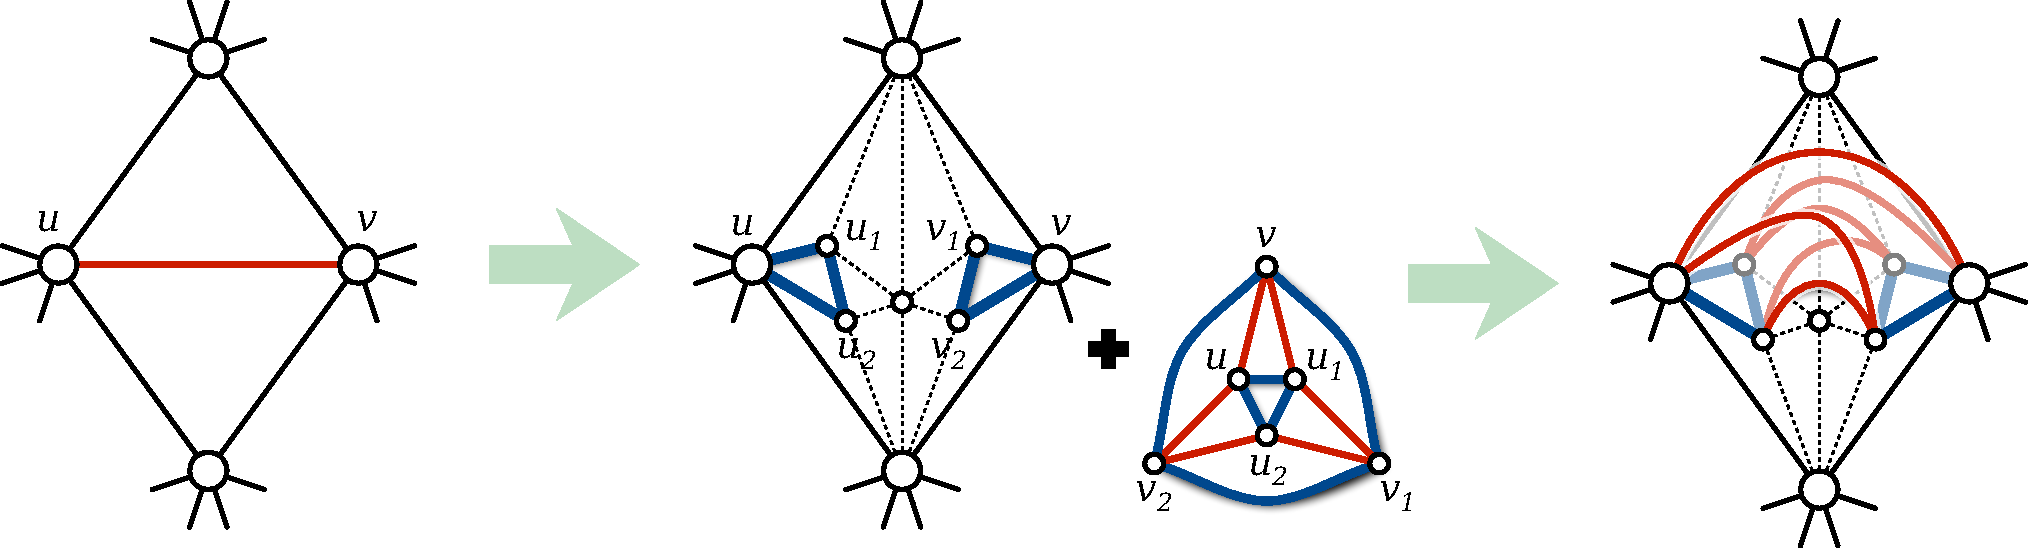
\includegraphics[height=2.25in]{Fig/addhandle3}
\caption{Adding a handle to transform a negative edge into a negative cocycle.  Thick (blue) edges have cost $C$; dashed edges have cost zero.}
\label{F:addhandle}
\end{figure}

Let $G'$ denote the transformed graph and $c'\colon E(G')\to \Real$ its associated cost function.  The minimum cut in $G'$ cannot contain any edge of an endpoint triangle.  Thus, for each edge cocycle, either all six edges cross the cut, or none of them cross the cut.  It follows that the minimum cut in $G'$ corresponds to a cut with equal cost in the original graph $G$.  Conversely, any cut in $G$ can be transformed into a cut in~$G'$ of equal cost.  Thus, computing the minimum cut in $G'$ is equivalent to computing the minimum cut in $G$.

\begin{theorem}
Given an even subgraph $H$ of an edge-weighted graph $G$ embedded on a surface without boundary, computing the minimum-weight even subgraph homologous to $H$ is strongly {NP}-hard.
\end{theorem}

Our reduction can be modified further to impose other desirable properties on the output instances, for example, that the graph is unweighted, every vertex has degree $3$, or the input subgraph $H$ is a simple cycle.
\note{kylejfox: There's a commented out note about how we can further reduce to $3^g$ instances of minimum $(s,t)$-cut in a graph of genus $O(g)$.
Do we want to put that back in?}
%Interestingly, any instance built by our reduction can be further reduced to $3^g$ instances of minimum $(s,t)$-cut in a graph of genus $O(g)$.  For each edge cocycle, we guess which sides of the cut contains its vertex triangles.  If they lie on different sides, we remove the handle, join the vertices on one vertex triangle to a common supersource~$s$, and join the vertices of the other vertex triangle to a common supersink~$t$.  (If they lie on the same side, we do nothing to the cocycle.)  After modifying the graph, we compute the minimum-cost $(s,t)$-cut.

Finally, we emphasize that the {NP}-hardness of this problem relies crucially on the fact that we are using homology with coefficients taken from the finite field $\Z_2$.  The corresponding problem for homology with real or integer coefficients is a minimum-cost circulation problem, and thus can be solved in polynomial time.
Chambers, Erickson and Nayyeri~\cite{cen-hfcc-12} show that this circulation problem can be solved in near-linear time for graphs of constant genus and polynomially bounded integer edge capacities using very different techniques.

\section{Global Minimum Cut}
\label{sec:global}

Let~$G$ be undirected. We now turn our attention computing the global minimum cut of~$G$.
To work with topology in computing a minimum cut, we use the following lemma which is similar very similar to Lemma~\ref{lem:cut-duality}.
We say a null-homologous even subgraph~$\eta$ is a \EMPH{separating subgraph} if it contains at least one edge.

\note{kylejfox: Throughout the dissertation I said vertex sets were cuts. We may need to reconcile with the $s,t$-cut papers.}
\begin{lemma}
\label{lem:mincut-z2}
Let~$G$ be an undirected graph with non-negative edge capacities, cellularly embedded on a surface~$\Sigma$ without boundary, let~$S$ be a minimum cut in~$G$, and let~$C$ be the edges crossing~$S$.  Then~$C^*$ is a minimum weight separating subgraph of~$G^*$.
\end{lemma}

\begin{proof}
  Let~$C$ be the edges crossing an arbitrary cut in~$G$.  The cut partitions the vertices of $G$
  into two disjoint subsets~$S$ and~$T$. Therefore, the dual subgraph~$C^*$
  partitions the faces of~$G^*$ into two disjoint subsets~$S^*$ and~$T^*$.
  Further,~$C^*$ is the boundary of the union of faces in~$S^*$, implying
  that~$C^*$ is null-homologous in~$\Sigma$ and therefore separating.

  Conversely, let~$C^*$ be an arbitrary separating subgraph of~$G^*$.
  As~$C^*$ is null-homologous, it is the boundary of a subset of the faces
  of~$G^*$.  Moreover, because $C^*$ is non-empty, it must be the boundary of
  a \emph{proper, non-empty} subset of faces.  Let $s^*$ and $t^*$ be faces
  of $G^*$ on either side of $C^*$.  Any path from~$s$ to~$t$ in the primal
  graph~$G$ must traverse at least one edge of~$C$.  We conclude that~$C$ crosses
  a cut (in particular, an $s,t$-cut).
\end{proof}

Fix an undirected graph~$G=(V,E)$, a non-negative weight function ${w\colon E\to \Real}$, and a cellular embedding of~$G$ on a surface~$\Sigma$ of genus~$g$ with at least two faces.  In light of Lemma \ref{lem:mincut-z2}, we focus our attention on finding a minimum weight separating subgraph of~$G$. 

Our algorithm separately considers two cases, illustrated in Figure~\ref{fig:global_cases}. Exactly one of these cases must apply to the minimum weight separating subgraph.
\begin{enumerate}
  \item
    Some minimum weight separating subgraph consists of a single contractible simple cycle.
  \item
    Every minimum weight separating subgraph can be decomposed into non-contractible simple cycles.
\end{enumerate}
%
\begin{figure}[h]
\centering
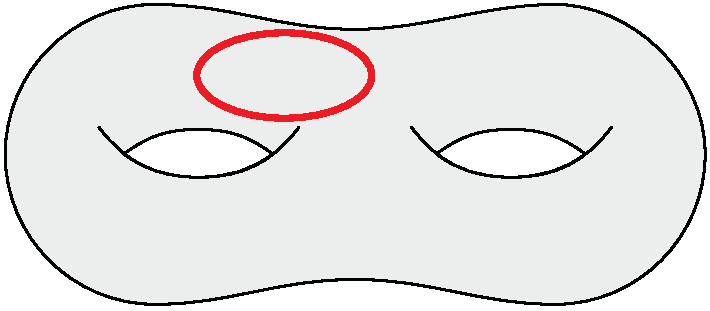
\includegraphics[height=1in]{Fig/shortcon2}\qquad
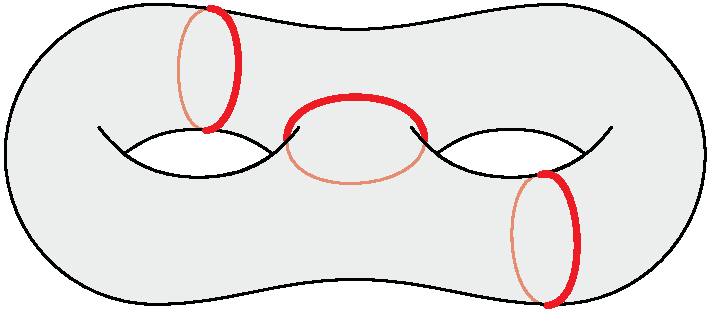
\includegraphics[height=1in]{Fig/homologous1}
\caption{Two types of minimum weight separating subgraphs: a contractible cycle and otherwise.}
\label{fig:global_cases}
\end{figure}
%

Throughout the rest of this section, we describe two subroutines to find minimum weight separating subgraphs that are designed with their corresponding condition in mind. If the corresponding condition does hold, the subroutine will return a separating subgraph with weight at most that of the minimum weight separating subgraph. Otherwise, the subroutine may return a higher weight separating subgraph. By running both subroutines and returning the best result, we find a minimum weight separating subgraph no matter which category it falls into.

%%%%%%%%%%%%%%%%%%%%%%%%%

\subsection{Contractible cycle}
\label{sec:global_contractible}

We begin by describing an algorithm to handle the case where some minimum weight separating subgraph is a contractible simple cycle.
We begin by borrowing a result of Cabello~\cite[Lemma 4.1]{c-fscss-10}.

\begin{lemma}[Cabello~\cite{c-fscss-10}]
\label{lem:disjoint-tight-arc}
Let $\alpha$ be a tight arc or tight cycle on $G$.  There exists a shortest contractible simple cycle that does not cross $\alpha$.
\end{lemma}

\begin{corollary}
\label{cor:disjoint-sep-cycle}
The shortest contractible simple cycle and the shortest non-separating cycle in $G$ do not cross.
\end{corollary}

\begin{figure}[h]
\centering
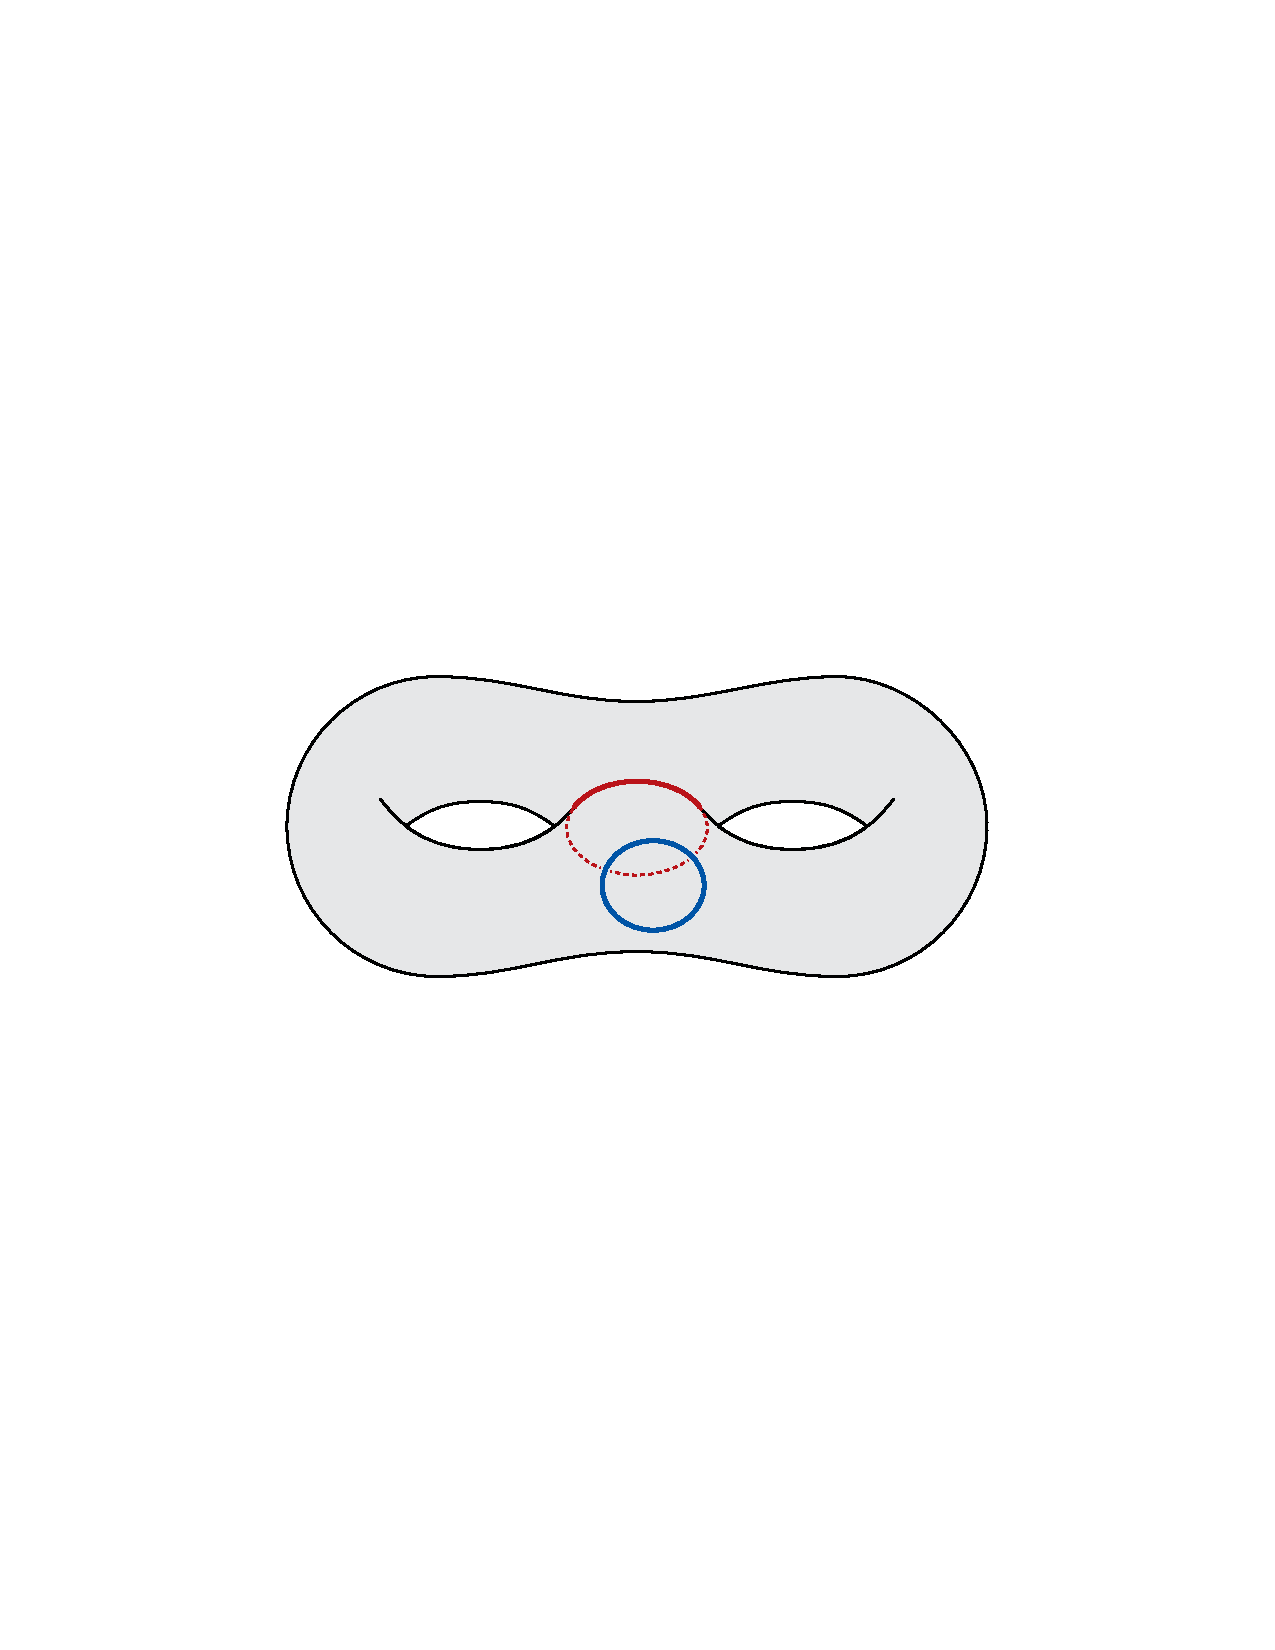
\includegraphics[height=1.2in]{Fig/shortcon-vs-shortnonsep}
\caption{A shortest contractible simple cycle does not cross some shortest non-separating cycle.}
\label{fig:global_shortcon-vs-shortnonsep}
\end{figure}

Cabello~\cite{c-fscss-10} uses these observations in order to compute a shortest contractible simple cycle in a surface embedded graph.
Unfortunately his algorithm takes~$\Omega(n^2)$ time, because his algorithm must return a shortest contractible simple cycle even if it is not a minimum weight separating subgraph.
Cabello \etal~\cite{cdem-fotc-10} use a similar procedure to find a shortest \emph{enclosing cycle} which bounds a non-empty set of faces.
While this procedure can be modified to run in~$g^{O(g)} n \log \log n$ time, it may return a cycle that is actually trivial after taking the symmetric difference over all its edges with multiplicity.
The cycle returned may not be a separating subgraph as per our definition.

Our algorithm will make use of the cutting operation ($\snip$) along tight cycles and arcs in~$G$.
\note{TODO: Define $\snip$ in the prelims.}
The following lemma implies it is safe for our algorithm to find minimum weight separating subgraphs in snipped copies of~$\Sigma$.
\begin{lemma}
\label{lem:global_null-homologous-projections}
Let~$\alpha$ be an arbitrary simple cycle or arc in~$G$. Let
${\Sigmasnip = \Sigma \snip \alpha}$ and let~$\Gsnip = G \snip \alpha$. Any null-homologous even subgraph~$\gammasnip$ in~$\Gsnip$ projects to a null-homologous even subgraph in~$G$.
\end{lemma}
\begin{proof}
Let~$\gammasnip$ be an arbitrary null-homologous even subgraph in~$\Gsnip$ and let~$\gamma$ be its projection in~$G$.
Subgraph~$\gamma$ bounds a subset of faces~$F_{\subsnip}$ in~$\Gsnip$. 
Let~$F$ be the projection of~$F_{\subsnip}$ into~$G$.
We will argue that~$\gamma$ bounds~$F$, proving the lemma.

Consider any edge~$e = f | g$ on the boundary of~$F$. If~$f$ and~$g$ still lie adjacent along~$e$ in~$\Gsnip$, then~$e$ bounds~$F_{\subsnip}$ and appears in~$\gamma$. If~$e$ separates a face~$f$ from the boundary of~$\Gsnip$, then~$e$ still appears in~$\gamma$.

Now consider any edge~$e$ in~$\gammasnip$. Suppose~$e$ does not lie along~$\alpha$ so that its projection appears in~$\gamma$. Edge~$e$ separates two faces~$f$ and~$g$ in~$\Gsnip$, and exactly one of those faces appears in~$F$. Now suppose~$e$ does lie along~$\alpha$. Edge~$e$ separates face~$f \in F$ from the boundary of~$\Gsnip$. The projection of~$e$ may separate~$f$ from another face~$g$. If~$g$ exists and is also in~$F$, then there exists another edge~$e'$ in~$\Gsnip$ that separates~$g$ from the boundary of~$\Gsnip$. The projections of~$e$ and~$e'$ cancel each other when taking the symmetric difference so their projection does not appear in~$\gamma$. Finally, if~$g$ does not exist or~$g$ is not a member of~$F$, then there is not another edge that shares a projection with~$e$. The projection of~$e$ will exist in~$\gamma$.
\end{proof}

We now present the main result of this section.
\begin{lemma}
\label{lem:contractible-alg}
There exists a~$g^{O(g)} n \log \log n$ time algorithm that computes a minimum weight separating subgraph if any such subgraph is a contractible simple cycle. If not, the algorithm either returns some separating subgraph (that may not be minimum weight) or nothing.
\end{lemma}

\begin{proof}
Our algorithm begins by computing a shortest non-separating cycle~$\alpha$ in $G$ in $g^{O(g)}n \log \log n$ time, using a modification of an algorithm of Kutz~\cite{k-csnco-06} by Italiano \etal~\cite{insw-iamcmf-11} or using a recent $2^{O(g)}n \log \log n$ time algorithm of Fox~\cite{f-sntcd-13}.  The surface $\Sigma \snip \alpha$ has two boundary cycles $\alpha'$ and $\alpha''$.

It then computes a system $P$ of tight arcs anchored on $\alpha'$ and $\alpha''$ in $O(n)$ time as described in Section~\ref{sec:characterizing_crossings}.
\note{Again, verify that the set of arcs can be computed in linear time this way.}
Let $\Gsnip$ denote the planar graph $G \snip (\alpha \cup P)$; this graph has $O(gn)$ vertices.

Pick an arbitrary edge $e$ of $\alpha$, and let $e_1$ and $e_2$ be distinct copies of $e$ in~$\Gsnip$.  Let $\gamma_1$ and $\gamma_2$ be the shortest simple cycles in the  subgraphs $\Gsnip \backslash e_1$ and $\Gsnip \backslash e_2$, respectively.  Our algorithm computes both~$\gamma_1$ and~$\gamma_2$ in $O(gn \log\log n)$ time using the algorithm of \L\c{a}cki and Sankowski~\cite{ls-mcsc-11}. Note that graphs~$\Gsnip \backslash e_1$ and~$\Gsnip \backslash e_2$ may not contain any cycles. In this case,~$\Gsnip$ contains no simple cycles. Corollary~\ref{cor:disjoint-sep-cycle} and Lemma~\ref{lem:disjoint-tight-arc} imply~$G$ does not contains any contractible simple cycles to begin with and our algorithm returns nothing. For the rest of this section, we assume~$\gamma_1$ and~$\gamma_2$ are well defined.

\begin{figure}[h]
\centering
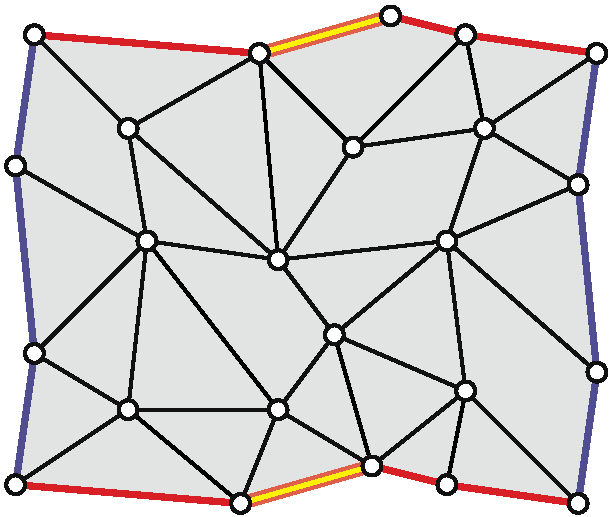
\includegraphics[height=1.2in]{Fig/forbidden-pair}
\caption{At least one copy of $e$ is forbidden in the planarized graph.}
\label{fig:global_forbidden-pair}
\end{figure}

Let~$\gamma$ be the shorter of the cycles~$\gamma_1$ and $\gamma_2$.  By multiple instantiations of Lemma~\ref{lem:global_null-homologous-projections}, cycle~$\gamma$ projects to a null-homologous closed walk $\gamma'$ in the original graph $G$, which may or may not be simple.
Our algorithm returns the symmetric difference over all edges in~$\gamma'$. The outer face of $\Gsnip$ is the only face that is not also a face of~$G$.
It follows that the only separating cycle in $\Gsnip$ that is not a separating subgraph in $G$ is the boundary of outer face.  Because $\gamma$ avoids at least one edge of the outer face, the carrier of $\gamma'$ must be non-empty. If our algorithm returns anything, it must return a separating subgraph.

Now, suppose some minimum weight separating subgraph of~$G$ is a contractible simple cycle. Corollary~\ref{cor:disjoint-sep-cycle} and Lemma~\ref{lem:disjoint-tight-arc} imply that some shortest contractible simple cycle $\sigma$ in $G$ crosses neither~$P$ nor $\alpha$.  (We emphasize that our algorithm does not necessarily compute~$\sigma$.)  This cycle $\sigma$ appears as a simple cycle in $\Gsnip$ that avoids at least one of the edges $e_1$ or $e_2$.  Thus, $\sigma$ cannot be shorter than $\gamma$, and our algorithm returns a minimum weight separating subgraph.
\end{proof}

%%%%%%%%%%%%%%%%%%%%%%%%%%%%%%%%%%%%

\subsection{Non-contractible components}
\label{sec:global_non-contractible}
Next, we consider the case where all minimum weight separating subgraphs contain components that are non-contractible. The following lemma is the key result of this section and could likely have applications beyond this work.
\begin{lemma}
\label{lem:global_split-nocross}
Let~$\sigma$ be a minimum weight separating subgraph, and let~$f$ be any face of~$G$.
Let~$\gamma$ be a closed walk on~$G$ that lies in the closure of the opposite component of~$f$ in~$\Sigma \setminus \sigma$, and let~$\eta$
be a shortest even subgraph homologous to~$\gamma$.
There exists a minimum weight separating subgraph~$\sigma'$ (possibly~$\sigma$) such
that~$\eta$ lies in the closure of the opposite component of~$f$ in~$\Sigma \setminus \sigma'$. (See Figure~\ref{fig:global_nonsep-vs-shortsep}.)
\end{lemma}
\begin{figure}[h]
\centering
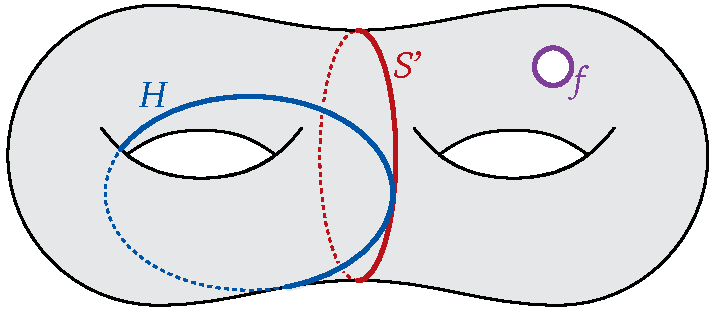
\includegraphics[height=1.2in]{Fig/nonsep-vs-shortsep}
\caption{The setting of Lemma~\ref{lem:global_split-nocross}. A~$\Z_2$-minimal even subgraph~$\eta$ is separated from face~$f$ by a minimum weight separating subgraph~$\sigma'$.}
\label{fig:global_nonsep-vs-shortsep}
\end{figure}
\begin{proof}
If~$\sigma$ fits the requirement that~$\eta$ lies in the closure of the opposite component of~$f$ in~$\Sigma \setminus \sigma$, then we are done. Assume otherwise.
The subgraph~$\sigma$ separates the faces of~$G$ into two non-empty sets.  Call the faces in the component of~$\Sigma \setminus \sigma$ containing~$f$ the \emph{far} faces and call the rest of the faces  \emph{near}.  Similarly, the even subgraph $\eta \oplus \gamma$ is null-homologous and separates the faces of $G$ into two subsets; call the faces in the subset containing~$f$ \emph{black} and the others \emph{white}.

Let~$\sigma'$ be the boundary of the union of the far black faces in $G$.
By definition,~$\sigma'$ is a null-homologous even subgraph.  By assumption, $\eta$ has edges that are incident to two far faces, but $\gamma$ does not; thus, there is at least one far black face~$f$.  Since there is also at least one near face, $\sigma'$ is non-empty. 
No edge of~$\eta$ lies between two far black faces so~$\eta$ lies in the closure of the opposite component of~$f$ in~$\Sigma \setminus \sigma'$. We claim~$\sigma'$ is a minimum weight even subgraph.

For the sake of contradiction, suppose~$\sigma'$ is not a minimum weight even subgraph.
Because both~$\sigma'$ and $\sigma$ are null-homologous, the even subgraph $\eta' = \eta \oplus \sigma' \oplus \sigma$ is homologous to $\eta$, and therefore to $\gamma$.

For any subgraph~$H$ of $G$, let $w(H)$ denote the sum of the weights of the edges of $H$.  We now prove that $w(\sigma') + w(\eta') \leq w(\eta) + w(\sigma)$ by bounding the contribution of each edge $e \in E(G)$ to both sides of the inequality.  Note that both $\sigma'$ and $\eta'$ are subgraphs of $\sigma\cup \eta$; moreover, $\sigma' \oplus \eta' = \sigma \oplus \eta$.  There are three cases to consider.
\begin{itemize}
\item
If $e \not\in \eta \cup \sigma$, then $e$ contributes $0$ to both sides of the inequality.
\item
If $e \in \sigma \oplus \eta$, then $e \in \sigma' \oplus \eta'$.  In this case, $e$ contributes $w(e)$ to both sides of the inequality.
\item
If $e \in \sigma \cap \eta$, then $e$ contributes exactly $2w(e)$ to the right side of the inequality.  Trivially, $e$ contributes at most $2w(e)$ to the left side.
\end{itemize}

On the other hand, because $\sigma'$ is not a minimum weight separating subgraph, we must have $w(\sigma') > w(\sigma)$. 
It immediately follows that $w(\eta') < w(\eta)$, which contradicts the minimality of $\eta$.
\end{proof}

We now present the main result of this section, concluding the description of our algorithm for computing minimum weight separating subgraphs and minimum cuts.
\begin{lemma}
  \label{lem:global_split-alg}
  There exists a~$g^{O(g)} n \log \log n$ time algorithm that computes a minimum weight separating subgraph if every minimum weight separating subgraph can be decomposed into non-contractible simple cycles. If not, the algorithm either returns some separating subgraph (that may not be minimum weight) or nothing.
\end{lemma}
\begin{proof}
Our algorithm begins by picking an arbitrary face~$f$ of~$G$. Let~$\sigma$ be an arbitrary minimum weight separating subgraph.
We argue that there exists a non-separating closed walk~$\gamma$ in~$G$ that lies in the closure of the opposite component of~$f$ in~$\Sigma \setminus \sigma$.

By assumption,~$\sigma$ can be decomposed into simple cycles, each of which is non-contractible. Suppose~$\sigma$ consists of more than one cycle. None of the cycles are null-homologous, because we could remove a single null-homologous cycle from~$\sigma$ to lower its cost without changing it homology class.
In this case,~$\gamma$ is simply one of the cycles in~$\sigma$'s decomposition. Now, assume~$\sigma$ consists of a single simple cycle. Cycle~$\sigma$ is not contractible by assumption, so neither component of $\Sigma \setminus \sigma$ is planar. The closure of the component opposite~$f$ has non-zero genus and therefore contains a non-separating closed walk in~$\Sigma$.

Let~$\eta$ be a shortest even subgraph homologous to~$\gamma$.
By Lemma~\ref{lem:global_split-nocross}, we may assume without loss of generality that~$\eta$ lies in the closure of the opposite component of~$f$ in~$\Sigma \setminus \sigma$. Assume for now that our algorithm knows~$\eta$. We will remove this assumption later in the proof.

Our algorithm picks an arbitrary edge~$e = h_1 | h_2$ of~$\eta$. At least one of~$h_1$ and~$h_2$ lies in the closure of the opposite component of~$f$ in~$\Sigma \setminus \sigma$. Our algorithm computes minimum weight subgraphs separating~$h_1$ from~$f$ and~$h_2$ from~$f$ using the minimum $s,t$-cut algorithm of Section~\ref{sec:crossing}. It then returns the cheaper of these two subgraphs, which weighs no more than~$\sigma$.

We now remove the assumption that our algorithm knows~$\eta$. Non-separating even subgraph~$\eta$ is shortest for one of~$2^{2g}-1$ homology classes. Our algorithm enumerates all~$2^{2g}-1$ homology classes by sampling subsets of cycles from a homology basis~\cite{e-dgteg-03}. For each homology class~$x$, it finds the shortest even subgraph~$\eta_x$ and runs the subroutine described in the previous paragraph assuming~$\eta = \eta_x$. If a there exists no subgraph separating the arbitrarily picked edge~$e \in \eta_x$ from~$f$ (in other words,~$e = f | f$), then the subroutine correctly returns nothing for that choice of homology class.
The algorithm returns the least weight separating subgraph returned by any instantiation of the subroutine or nothing if no instantiation returns a separating subgraph.
One of the homology classes contains~$\eta$, so the algorithm will eventually find the minimum weight separating subgraph assuming every minimum weight separating subgraph can be decomposed into non-contractible simple cycles.
\end{proof}

By running the algorithms described in Lemmas~\ref{lem:contractible-alg} and~\ref{lem:global_split-alg}, we get the main results of this section.

\begin{theorem}
Let $G$ be an edge-weighted undirected graph embedded on a surface with genus $g$.
We can compute a minimum-weight separating subgraph in $G$ in $g^{O(g)} n \log \log n$ time.
\end{theorem}

\begin{corollary}
Let $G$ be an edge-weighted undirected graph embedded on a surface with genus $g$.
We can compute a global minimum cut in $G$ in $g^{O(g)} n \log \log n$ time.
\end{corollary}

\section{Conclusions and Open Problems}

\note{TODO: Write a section on conclusions and open problems.}



% Begin bbl nonsense
\bibliographystyle{abbrv}
\bibliography{topology,data-structures,optimization,other}


\end{document}
